\documentclass[twoside]{book}

% Packages required by doxygen
\usepackage{calc}
\usepackage{doxygen}
\usepackage{graphicx}
\usepackage[utf8]{inputenc}
\usepackage{makeidx}
\usepackage{multicol}
\usepackage{multirow}
\usepackage{textcomp}
\usepackage[table]{xcolor}

% Font selection
\usepackage[T1]{fontenc}
\usepackage{mathptmx}
\usepackage[scaled=.90]{helvet}
\usepackage{courier}
\usepackage{amssymb}
\usepackage{sectsty}
\renewcommand{\familydefault}{\sfdefault}
\allsectionsfont{%
  \fontseries{bc}\selectfont%
  \color{darkgray}%
}
\renewcommand{\DoxyLabelFont}{%
  \fontseries{bc}\selectfont%
  \color{darkgray}%
}

% Page & text layout
\usepackage{geometry}
\geometry{%
  a4paper,%
  top=2.5cm,%
  bottom=2.5cm,%
  left=2.5cm,%
  right=2.5cm%
}
\tolerance=750
\hfuzz=15pt
\hbadness=750
\setlength{\emergencystretch}{15pt}
\setlength{\parindent}{0cm}
\setlength{\parskip}{0.2cm}
\makeatletter
\renewcommand{\paragraph}{%
  \@startsection{paragraph}{4}{0ex}{-1.0ex}{1.0ex}{%
    \normalfont\normalsize\bfseries\SS@parafont%
  }%
}
\renewcommand{\subparagraph}{%
  \@startsection{subparagraph}{5}{0ex}{-1.0ex}{1.0ex}{%
    \normalfont\normalsize\bfseries\SS@subparafont%
  }%
}
\makeatother

% Headers & footers
\usepackage{fancyhdr}
\pagestyle{fancyplain}
\fancyhead[LE]{\fancyplain{}{\bfseries\thepage}}
\fancyhead[CE]{\fancyplain{}{}}
\fancyhead[RE]{\fancyplain{}{\bfseries\leftmark}}
\fancyhead[LO]{\fancyplain{}{\bfseries\rightmark}}
\fancyhead[CO]{\fancyplain{}{}}
\fancyhead[RO]{\fancyplain{}{\bfseries\thepage}}
\fancyfoot[LE]{\fancyplain{}{}}
\fancyfoot[CE]{\fancyplain{}{}}
\fancyfoot[RE]{\fancyplain{}{\bfseries\scriptsize Generated on Mon Feb 25 2019 17\-:01\-:26 for Molssi Driver Interface Library by Doxygen }}
\fancyfoot[LO]{\fancyplain{}{\bfseries\scriptsize Generated on Mon Feb 25 2019 17\-:01\-:26 for Molssi Driver Interface Library by Doxygen }}
\fancyfoot[CO]{\fancyplain{}{}}
\fancyfoot[RO]{\fancyplain{}{}}
\renewcommand{\footrulewidth}{0.4pt}
\renewcommand{\chaptermark}[1]{%
  \markboth{#1}{}%
}
\renewcommand{\sectionmark}[1]{%
  \markright{\thesection\ #1}%
}

% Indices & bibliography
\usepackage{natbib}
\usepackage[titles]{tocloft}
\setcounter{tocdepth}{3}
\setcounter{secnumdepth}{5}
\makeindex

% Hyperlinks (required, but should be loaded last)
\usepackage{ifpdf}
\ifpdf
  \usepackage[pdftex,pagebackref=true]{hyperref}
\else
  \usepackage[ps2pdf,pagebackref=true]{hyperref}
\fi
\hypersetup{%
  colorlinks=true,%
  linkcolor=blue,%
  citecolor=blue,%
  unicode%
}

% Custom commands
\newcommand{\clearemptydoublepage}{%
  \newpage{\pagestyle{empty}\cleardoublepage}%
}


%===== C O N T E N T S =====

\begin{document}

% Titlepage & ToC
\hypersetup{pageanchor=false}
\pagenumbering{roman}
\begin{titlepage}
\vspace*{7cm}
\begin{center}%
{\Large Molssi Driver Interface Library }\\
\vspace*{1cm}
{\large Generated by Doxygen 1.8.5}\\
\vspace*{0.5cm}
{\small Mon Feb 25 2019 17:01:26}\\
\end{center}
\end{titlepage}
\clearemptydoublepage
\tableofcontents
\clearemptydoublepage
\pagenumbering{arabic}
\hypersetup{pageanchor=true}

%--- Begin generated contents ---
\chapter{Main Page}
\label{index}\hypertarget{index}{}\hypertarget{index_overview_sec}{}\section{Overview}\label{index_overview_sec}
The Mol\-S\-S\-I Driver Interface (M\-D\-I) library enables codes to interoperate via the M\-D\-I.\hypertarget{index_source_sec}{}\section{Source Code}\label{index_source_sec}
The source code of the M\-D\-I library is available at Git\-Hub at \href{https://github.com/MolSSI/molssi_driver_interface}{\tt https\-://github.\-com/\-Mol\-S\-S\-I/molssi\-\_\-driver\-\_\-interface}\hypertarget{index_commands_sec}{}\section{M\-D\-I Standard}\label{index_commands_sec}
\hypertarget{index_command_list}{}\subsection{Command List}\label{index_command_list}
The following is a list of commands that are officially part of the M\-D\-I standard.\hypertarget{index_set_cell}{}\subsubsection{$>$\-C\-E\-L\-L}\label{index_set_cell}
The driver sends a set of cell vectors to the engine, which immediately resizes its simulation cell to the dimensions specified by the cell vectors. In the case of a quantum chemistry code that uses a plane wave basis set, the engine will either immediately recalculate the g-\/vectors or schedule the g-\/vectors to be recalculated at the beginning of the next S\-C\-F command.\hypertarget{index_recv_cell}{}\subsubsection{$<$\-C\-E\-L\-L}\label{index_recv_cell}
The engine sends a set of cell vectors to the driver, in the same format as specified for the {\ttfamily $>$C\-E\-L\-L} command.\hypertarget{index_send_charges}{}\subsubsection{$>$\-C\-H\-A\-R\-G\-E\-S}\label{index_send_charges}
The driver sends a set of atomic charges to the engine, which immediately changes its atomic charges to those sent by the driver. The charges are represented by double precision floats. The number of values sent is equal to the response to the $<$N\-A\-T\-O\-M\-S command. The charges are provided in sequentially ascending order of atomic index.\hypertarget{index_recv_charges}{}\subsubsection{$<$\-C\-H\-A\-R\-G\-E\-S}\label{index_recv_charges}
The engine sends a set of atomic charges to the driver, in the same format as specified for the {\ttfamily $>$C\-H\-A\-R\-G\-E\-S} command.\hypertarget{index_send_coords}{}\subsubsection{$<$\-C\-O\-O\-R\-D\-S}\label{index_send_coords}
The driver sends a set of atomic coordinates to the engine, which immediately changes its atomic coordinates to those sent by the driver. The coordinates are represented by double precision floats. The number of values sent is equal to three times the response to the $<$N\-A\-T\-O\-M\-S command. The coordinates for each atom are provided in sequentially ascending order of atomic index, with the coordinates for each individual atom being provided in xyz order.\hypertarget{index_send_coords}{}\subsubsection{$<$\-C\-O\-O\-R\-D\-S}\label{index_send_coords}
The engine sends a set of atomic coordinates to the driver, in the same format as specified for the {\ttfamily $>$C\-O\-O\-R\-D\-S} command.\hypertarget{index_recv_energy}{}\subsubsection{$<$\-E\-N\-E\-R\-G\-Y}\label{index_recv_energy}
The engine sends its most recently calculated energy to the driver. The {\ttfamily M\-D\-\_\-\-I\-N\-I\-T}, {\ttfamily S\-C\-F}, and {\ttfamily T\-I\-M\-E\-S\-T\-E\-P} commands can be used to cause the engine to calculate a new energy.\hypertarget{index_exit_command}{}\subsubsection{E\-X\-I\-T}\label{index_exit_command}
The engine terminates and can no longer be sent commands.\hypertarget{index_send_forces}{}\subsubsection{$>$\-F\-O\-R\-C\-E\-S}\label{index_send_forces}
The driver sends a set of atomic forces to the engine, in the same format specified by the {\ttfamily $>$C\-O\-O\-R\-D\-S} command. If a {\ttfamily T\-I\-M\-E\-S\-T\-E\-P} command is later sent to the engine, {\bfseries  after any normal calculation of forces and immediately prior to time integration}, the engine will replace its internal forces with the forces sent by the driver.\hypertarget{index_send_add_forces}{}\subsubsection{$>$+\-F\-O\-R\-C\-E\-S}\label{index_send_add_forces}
As {\ttfamily $>$F\-O\-R\-C\-E\-S}, except that instead of replacing its internal forces with those sent by the driver, the engine adds the forces sent by the driver to its internal forces.\hypertarget{index_recv_forces}{}\subsubsection{$<$\-F\-O\-R\-C\-E\-S}\label{index_recv_forces}
The engine calculates and sends a set of atomic forces to the driver, in the same format specified by the {\ttfamily $>$C\-O\-O\-R\-D\-S} command. These forces include all force contributions, including the force contributions associated with any constraint algorithm (e.\-g. S\-H\-A\-K\-E, R\-A\-T\-T\-L\-E, etc.).\hypertarget{index_recv_masses}{}\subsubsection{$<$\-M\-A\-S\-S\-E\-S}\label{index_recv_masses}
The engine sends the driver the mass of each of the atom types. The masses are represented by double precision floats. The number of values sent is equal to response to the $<$N\-T\-Y\-P\-E\-S command. The values are provided in sequentially ascending order of type index (see the {\ttfamily $<$T\-Y\-P\-E\-S} command).\hypertarget{index_md_init}{}\subsubsection{M\-D\-\_\-\-I\-N\-I\-T}\label{index_md_init}
The engine performs any initialization operations that are necessary before an M\-D simulation can be time propagated. These initialization operations {\bfseries  may change the engine's atomic coordinates } under certain circumstances, such as if the S\-H\-A\-K\-E algorithm is used. This engine calculates the energy of the system, which can be queried by the {\ttfamily $<$E\-N\-E\-R\-G\-Y} command.\hypertarget{index_send_name}{}\subsubsection{$<$\-N\-A\-M\-E}\label{index_send_name}
The engine sends the driver a string of length {\ttfamily M\-D\-I\-\_\-\-N\-A\-M\-E\-\_\-\-L\-E\-N\-G\-T\-H} that corresponds to the argument of {\ttfamily -\/name} in the M\-D\-I initialization options. This argument allows a driver to identify the purpose of connected engine codes within the simulation. For example, a particular Q\-M/\-M\-M driver might require a connection with a single M\-M code and a single Q\-M code, with the expected name of the M\-M code being \char`\"{}\-M\-M\char`\"{} and the expected name of the Q\-M code being \char`\"{}\-Q\-M\char`\"{}. After initializing M\-D\-I and accepting communicators to the engines, the driver can use this command to identify which of the engines is the M\-M code and which is the Q\-M code.\hypertarget{index_recv_natoms}{}\subsubsection{$<$\-N\-A\-T\-O\-M\-S}\label{index_recv_natoms}
The engine sends the driver a single integer corresponding to the number of atoms in the engine's system.\hypertarget{index_recv_types}{}\subsubsection{$<$\-N\-T\-Y\-P\-E\-S}\label{index_recv_types}
The engine sends the driver a single integer corresponding to the number of different types of atoms (e.\-g. \char`\"{}\-H\char`\"{}, \char`\"{}\-He\char`\"{}, \char`\"{}\-C\char`\"{}, \char`\"{}\-O\char`\"{}, etc.) in the engine's system.\hypertarget{index_nuclear_step}{}\subsubsection{A\-T\-O\-M\-I\-C\-\_\-\-S\-T\-E\-P}\label{index_nuclear_step}
The engine performs a time propagation step for the nuclear coordinates.\hypertarget{index_send_preforces}{}\subsubsection{$>$\-P\-R\-E-\/\-F\-O\-R\-C\-E\-S}\label{index_send_preforces}
The driver sends a set of atomic forces to the engine, in the same format specified by the {\ttfamily $>$C\-O\-O\-R\-D\-S} command. If a {\ttfamily T\-I\-M\-E\-S\-T\-E\-P} command is later sent to the engine, {\bfseries  after calculation of all forces except those related to constraint algorithms (e.\-g. S\-H\-A\-K\-E, R\-A\-T\-T\-L\-E, etc.) and prior to application of any constraint algorithms}, the engine will replace its internal forces with the forces sent by the driver.\hypertarget{index_send_add_preforces}{}\subsubsection{$>$+\-P\-R\-E-\/\-F\-O\-R\-C\-E\-S}\label{index_send_add_preforces}
As {\ttfamily $>$P\-R\-E-\/\-F\-O\-R\-C\-E\-S}, except that instead of replacing its internal forces with those sent by the driver, the engine adds the forces sent by the driver to its internal forces.\hypertarget{index_recv_preforces}{}\subsubsection{$<$\-P\-R\-E-\/\-F\-O\-R\-C\-E\-S}\label{index_recv_preforces}
The engine calculates and sends a set of atomic forces to the driver, in the same format specified by the {\ttfamily $>$C\-O\-O\-R\-D\-S} command. These forces include all force contributions except those related to constraint algorithms (e.\-g. S\-H\-A\-K\-E, R\-A\-T\-T\-L\-E, etc.).\hypertarget{index_scf_command}{}\subsubsection{S\-C\-F}\label{index_scf_command}
The engine performs a full self-\/consistent field calculation in order to relax the electronic density distribution. The engine updates its energy, which can be queried with the {\ttfamily $<$E\-N\-E\-R\-G\-Y} command. 
\chapter{Namespace Index}
\doxysection{Namespace List}
Here is a list of all documented namespaces with brief descriptions\+:\begin{DoxyCompactList}
\item\contentsline{section}{\mbox{\hyperlink{namespaceMDI__Library_1_1mdi}{M\+D\+I\+\_\+\+Library.\+mdi}} }{\pageref{namespaceMDI__Library_1_1mdi}}{}
\item\contentsline{section}{\mbox{\hyperlink{namespaceMDI__Library_1_1mdi__mpi4py}{M\+D\+I\+\_\+\+Library.\+mdi\+\_\+mpi4py}} }{\pageref{namespaceMDI__Library_1_1mdi__mpi4py}}{}
\end{DoxyCompactList}

\chapter{Hierarchical Index}
\section{Class Hierarchy}
This inheritance list is sorted roughly, but not completely, alphabetically\-:\begin{DoxyCompactList}
\item \contentsline{section}{Communicator}{\pageref{classCommunicator}}{}
\begin{DoxyCompactList}
\item \contentsline{section}{Communicator\-M\-P\-I}{\pageref{classCommunicatorMPI}}{}
\item \contentsline{section}{Communicator\-T\-C\-P}{\pageref{classCommunicatorTCP}}{}
\end{DoxyCompactList}
\item \contentsline{section}{mdi}{\pageref{classmdi}}{}
\item \contentsline{section}{mdi\-:\-:M\-D\-I\-\_\-\-Accept\-\_\-\-Communicator\-\_\-}{\pageref{interfacemdi_1_1MDI__Accept__Communicator__}}{}
\item \contentsline{section}{mdi\-:\-:M\-D\-I\-\_\-\-Conversion\-\_\-\-Factor\-\_\-}{\pageref{interfacemdi_1_1MDI__Conversion__Factor__}}{}
\item \contentsline{section}{mdi\-:\-:M\-D\-I\-\_\-\-Init\-\_\-}{\pageref{interfacemdi_1_1MDI__Init__}}{}
\item \contentsline{section}{mdi\-:\-:mdi\-\_\-recv}{\pageref{interfacemdi_1_1mdi__recv}}{}
\item \contentsline{section}{mdi\-:\-:M\-D\-I\-\_\-\-Recv\-\_\-}{\pageref{interfacemdi_1_1MDI__Recv__}}{}
\item \contentsline{section}{mdi\-:\-:M\-D\-I\-\_\-\-Recv\-\_\-\-Command\-\_\-}{\pageref{interfacemdi_1_1MDI__Recv__Command__}}{}
\item \contentsline{section}{mdi\-:\-:mdi\-\_\-send}{\pageref{interfacemdi_1_1mdi__send}}{}
\item \contentsline{section}{mdi\-:\-:M\-D\-I\-\_\-\-Send\-\_\-}{\pageref{interfacemdi_1_1MDI__Send__}}{}
\item \contentsline{section}{mdi\-:\-:M\-D\-I\-\_\-\-Send\-\_\-\-Command\-\_\-}{\pageref{interfacemdi_1_1MDI__Send__Command__}}{}
\item \contentsline{section}{M\-D\-I\-Manager}{\pageref{classMDIManager}}{}
\item \contentsline{section}{Method\-M\-P\-I}{\pageref{classMethodMPI}}{}
\item \contentsline{section}{Method\-T\-C\-P}{\pageref{classMethodTCP}}{}
\end{DoxyCompactList}

\chapter{Class Index}
\section{Class List}
Here are the classes, structs, unions and interfaces with brief descriptions\-:\begin{DoxyCompactList}
\item\contentsline{section}{\hyperlink{classCommunicator}{Communicator} }{\pageref{classCommunicator}}{}
\item\contentsline{section}{\hyperlink{classCommunicatorMPI}{Communicator\-M\-P\-I} }{\pageref{classCommunicatorMPI}}{}
\item\contentsline{section}{\hyperlink{classCommunicatorTCP}{Communicator\-T\-C\-P} }{\pageref{classCommunicatorTCP}}{}
\item\contentsline{section}{\hyperlink{classmdi}{mdi} }{\pageref{classmdi}}{}
\item\contentsline{section}{\hyperlink{interfacemdi_1_1MDI__Accept__Communicator__}{mdi\-::\-M\-D\-I\-\_\-\-Accept\-\_\-\-Communicator\-\_\-} }{\pageref{interfacemdi_1_1MDI__Accept__Communicator__}}{}
\item\contentsline{section}{\hyperlink{interfacemdi_1_1MDI__Conversion__Factor__}{mdi\-::\-M\-D\-I\-\_\-\-Conversion\-\_\-\-Factor\-\_\-} }{\pageref{interfacemdi_1_1MDI__Conversion__Factor__}}{}
\item\contentsline{section}{\hyperlink{interfacemdi_1_1MDI__Init__}{mdi\-::\-M\-D\-I\-\_\-\-Init\-\_\-} }{\pageref{interfacemdi_1_1MDI__Init__}}{}
\item\contentsline{section}{\hyperlink{interfacemdi_1_1mdi__recv}{mdi\-::mdi\-\_\-recv} }{\pageref{interfacemdi_1_1mdi__recv}}{}
\item\contentsline{section}{\hyperlink{interfacemdi_1_1MDI__Recv__}{mdi\-::\-M\-D\-I\-\_\-\-Recv\-\_\-} }{\pageref{interfacemdi_1_1MDI__Recv__}}{}
\item\contentsline{section}{\hyperlink{interfacemdi_1_1MDI__Recv__Command__}{mdi\-::\-M\-D\-I\-\_\-\-Recv\-\_\-\-Command\-\_\-} }{\pageref{interfacemdi_1_1MDI__Recv__Command__}}{}
\item\contentsline{section}{\hyperlink{interfacemdi_1_1mdi__send}{mdi\-::mdi\-\_\-send} }{\pageref{interfacemdi_1_1mdi__send}}{}
\item\contentsline{section}{\hyperlink{interfacemdi_1_1MDI__Send__}{mdi\-::\-M\-D\-I\-\_\-\-Send\-\_\-} }{\pageref{interfacemdi_1_1MDI__Send__}}{}
\item\contentsline{section}{\hyperlink{interfacemdi_1_1MDI__Send__Command__}{mdi\-::\-M\-D\-I\-\_\-\-Send\-\_\-\-Command\-\_\-} }{\pageref{interfacemdi_1_1MDI__Send__Command__}}{}
\end{DoxyCompactList}

\chapter{File Index}
\section{File List}
Here is a list of all documented files with brief descriptions\-:\begin{DoxyCompactList}
\item\contentsline{section}{/home/tbarnes/mdi/molssi\-\_\-driver\-\_\-interface/molssi\-\_\-driver\-\_\-interface/\hyperlink{communicator_8cpp}{communicator.\-cpp} \\*Class definition for handling communication between connect codes }{\pageref{communicator_8cpp}}{}
\item\contentsline{section}{/home/tbarnes/mdi/molssi\-\_\-driver\-\_\-interface/molssi\-\_\-driver\-\_\-interface/\hyperlink{communicator_8h}{communicator.\-h} \\*Class declaration for handling communication between connected codes }{\pageref{communicator_8h}}{}
\item\contentsline{section}{/home/tbarnes/mdi/molssi\-\_\-driver\-\_\-interface/molssi\-\_\-driver\-\_\-interface/\hyperlink{mdi_8cpp}{mdi.\-cpp} \\*Functions callable by users of the Mol\-S\-S\-I Driver Interface }{\pageref{mdi_8cpp}}{}
\item\contentsline{section}{/home/tbarnes/mdi/molssi\-\_\-driver\-\_\-interface/molssi\-\_\-driver\-\_\-interface/{\bfseries mdi.\-h} }{\pageref{mdi_8h}}{}
\item\contentsline{section}{/home/tbarnes/mdi/molssi\-\_\-driver\-\_\-interface/molssi\-\_\-driver\-\_\-interface/\hyperlink{mdi__manager_8cpp}{mdi\-\_\-manager.\-cpp} \\*Class definition for top-\/level manager of M\-D\-I operations }{\pageref{mdi__manager_8cpp}}{}
\item\contentsline{section}{/home/tbarnes/mdi/molssi\-\_\-driver\-\_\-interface/molssi\-\_\-driver\-\_\-interface/\hyperlink{mdi__manager_8h}{mdi\-\_\-manager.\-h} \\*Class declaration for top-\/level manager of M\-D\-I operations }{\pageref{mdi__manager_8h}}{}
\item\contentsline{section}{/home/tbarnes/mdi/molssi\-\_\-driver\-\_\-interface/molssi\-\_\-driver\-\_\-interface/\hyperlink{method_8cpp}{method.\-cpp} \\*Class definition for top-\/level manager of M\-D\-I operations }{\pageref{method_8cpp}}{}
\item\contentsline{section}{/home/tbarnes/mdi/molssi\-\_\-driver\-\_\-interface/molssi\-\_\-driver\-\_\-interface/\hyperlink{method_8h}{method.\-h} \\*Class declaration for top-\/level manager of M\-D\-I operations }{\pageref{method_8h}}{}
\end{DoxyCompactList}

\chapter{Namespace Documentation}
\hypertarget{namespacemolssi__driver__interface_1_1mdi}{\section{molssi\-\_\-driver\-\_\-interface.\-mdi Namespace Reference}
\label{namespacemolssi__driver__interface_1_1mdi}\index{molssi\-\_\-driver\-\_\-interface.\-mdi@{molssi\-\_\-driver\-\_\-interface.\-mdi}}
}
\subsection*{Functions}
\begin{DoxyCompactItemize}
\item 
\hypertarget{namespacemolssi__driver__interface_1_1mdi_a7fa45893a21039fbc4f4558adff09247}{def {\bfseries M\-D\-I\-\_\-\-Init}}\label{namespacemolssi__driver__interface_1_1mdi_a7fa45893a21039fbc4f4558adff09247}

\item 
\hypertarget{namespacemolssi__driver__interface_1_1mdi_a13123f38cd87a7834a1686f3620b26f5}{def {\bfseries M\-D\-I\-\_\-\-Get\-\_\-\-Intra\-\_\-\-Code\-\_\-\-M\-P\-I\-\_\-\-Comm}}\label{namespacemolssi__driver__interface_1_1mdi_a13123f38cd87a7834a1686f3620b26f5}

\item 
\hypertarget{namespacemolssi__driver__interface_1_1mdi_a6491914c9c4bb9d3818f53895a735625}{def {\bfseries M\-D\-I\-\_\-\-Accept\-\_\-\-Communicator}}\label{namespacemolssi__driver__interface_1_1mdi_a6491914c9c4bb9d3818f53895a735625}

\item 
\hypertarget{namespacemolssi__driver__interface_1_1mdi_a75666a1612c8fde657f9783f3c42fcaf}{def {\bfseries M\-D\-I\-\_\-\-Send}}\label{namespacemolssi__driver__interface_1_1mdi_a75666a1612c8fde657f9783f3c42fcaf}

\item 
\hypertarget{namespacemolssi__driver__interface_1_1mdi_aad08bf01bdb806196e9a41140325b6ae}{def {\bfseries M\-D\-I\-\_\-\-Recv}}\label{namespacemolssi__driver__interface_1_1mdi_aad08bf01bdb806196e9a41140325b6ae}

\item 
\hypertarget{namespacemolssi__driver__interface_1_1mdi_a09f3c593e5222f1adbec84021f2b3f34}{def {\bfseries M\-D\-I\-\_\-\-Send\-\_\-\-Command}}\label{namespacemolssi__driver__interface_1_1mdi_a09f3c593e5222f1adbec84021f2b3f34}

\item 
\hypertarget{namespacemolssi__driver__interface_1_1mdi_aad3f7850b204cc18683005d43797bebc}{def {\bfseries M\-D\-I\-\_\-\-Recv\-\_\-\-Command}}\label{namespacemolssi__driver__interface_1_1mdi_aad3f7850b204cc18683005d43797bebc}

\end{DoxyCompactItemize}
\subsection*{Variables}
\begin{DoxyCompactItemize}
\item 
\hypertarget{namespacemolssi__driver__interface_1_1mdi_a659f7f2c2dad27268542893627dddd76}{tuple {\bfseries dir\-\_\-path} = os.\-path.\-dirname(os.\-path.\-realpath(\-\_\-\-\_\-file\-\_\-\-\_\-))}\label{namespacemolssi__driver__interface_1_1mdi_a659f7f2c2dad27268542893627dddd76}

\item 
\hypertarget{namespacemolssi__driver__interface_1_1mdi_ab641655ae2e8ddbbf84bea8e8e5bf953}{{\bfseries use\-\_\-numpy} = True}\label{namespacemolssi__driver__interface_1_1mdi_ab641655ae2e8ddbbf84bea8e8e5bf953}

\item 
\hypertarget{namespacemolssi__driver__interface_1_1mdi_a2d2043c182591fed4963dbcb9cf30484}{{\bfseries use\-\_\-mpi4py} = True}\label{namespacemolssi__driver__interface_1_1mdi_a2d2043c182591fed4963dbcb9cf30484}

\item 
\hypertarget{namespacemolssi__driver__interface_1_1mdi_ab47fd48619ba8e2bfe10f6d86d5be1b5}{tuple {\bfseries mdi\-\_\-name\-\_\-file} = open(dir\-\_\-path + \char`\"{}/mdi\-\_\-name\char`\"{},\char`\"{}r\char`\"{})}\label{namespacemolssi__driver__interface_1_1mdi_ab47fd48619ba8e2bfe10f6d86d5be1b5}

\item 
\hypertarget{namespacemolssi__driver__interface_1_1mdi_afc7bde19c202368b68fce956fdbc9035}{tuple {\bfseries mdi\-\_\-name} = mdi\-\_\-name\-\_\-file.\-read()}\label{namespacemolssi__driver__interface_1_1mdi_afc7bde19c202368b68fce956fdbc9035}

\item 
\hypertarget{namespacemolssi__driver__interface_1_1mdi_a57cb628499747477003d54de706ab429}{tuple {\bfseries mdi} = ctypes.\-C\-D\-L\-L(dir\-\_\-path + \char`\"{}/\char`\"{} + mdi\-\_\-name)}\label{namespacemolssi__driver__interface_1_1mdi_a57cb628499747477003d54de706ab429}

\item 
\hypertarget{namespacemolssi__driver__interface_1_1mdi_aa92fd47513f406f91b87c70b9dd221c6}{tuple {\bfseries M\-D\-I\-\_\-\-C\-O\-M\-M\-A\-N\-D\-\_\-\-L\-E\-N\-G\-T\-H} = ctypes.\-c\-\_\-int.\-in\-\_\-dll(\hyperlink{classmdi}{mdi}, \char`\"{}M\-D\-I\-\_\-\-C\-O\-M\-M\-A\-N\-D\-\_\-\-L\-E\-N\-G\-T\-H\char`\"{})}\label{namespacemolssi__driver__interface_1_1mdi_aa92fd47513f406f91b87c70b9dd221c6}

\item 
\hypertarget{namespacemolssi__driver__interface_1_1mdi_a3be426ffa2c8696fe44d1bec166a21a8}{tuple {\bfseries M\-D\-I\-\_\-\-N\-A\-M\-E\-\_\-\-L\-E\-N\-G\-T\-H} = ctypes.\-c\-\_\-int.\-in\-\_\-dll(\hyperlink{classmdi}{mdi}, \char`\"{}M\-D\-I\-\_\-\-N\-A\-M\-E\-\_\-\-L\-E\-N\-G\-T\-H\char`\"{})}\label{namespacemolssi__driver__interface_1_1mdi_a3be426ffa2c8696fe44d1bec166a21a8}

\item 
\hypertarget{namespacemolssi__driver__interface_1_1mdi_a451ed61cd0edd447d5a559ec99d479d5}{tuple {\bfseries M\-D\-I\-\_\-\-I\-N\-T} = ctypes.\-c\-\_\-int.\-in\-\_\-dll(\hyperlink{classmdi}{mdi}, \char`\"{}M\-D\-I\-\_\-\-I\-N\-T\char`\"{})}\label{namespacemolssi__driver__interface_1_1mdi_a451ed61cd0edd447d5a559ec99d479d5}

\item 
\hypertarget{namespacemolssi__driver__interface_1_1mdi_a52d5a1823d4b38b60df486d5b7a76d83}{tuple {\bfseries M\-D\-I\-\_\-\-D\-O\-U\-B\-L\-E} = ctypes.\-c\-\_\-int.\-in\-\_\-dll(\hyperlink{classmdi}{mdi}, \char`\"{}M\-D\-I\-\_\-\-D\-O\-U\-B\-L\-E\char`\"{})}\label{namespacemolssi__driver__interface_1_1mdi_a52d5a1823d4b38b60df486d5b7a76d83}

\item 
\hypertarget{namespacemolssi__driver__interface_1_1mdi_a2f9bb33fbf05ad85f489344f098c19e4}{tuple {\bfseries M\-D\-I\-\_\-\-C\-H\-A\-R} = ctypes.\-c\-\_\-int.\-in\-\_\-dll(\hyperlink{classmdi}{mdi}, \char`\"{}M\-D\-I\-\_\-\-C\-H\-A\-R\char`\"{})}\label{namespacemolssi__driver__interface_1_1mdi_a2f9bb33fbf05ad85f489344f098c19e4}

\item 
\hypertarget{namespacemolssi__driver__interface_1_1mdi_a30427c26974ad9a7bca4651b4a347896}{tuple {\bfseries M\-D\-I\-\_\-\-I\-N\-T\-\_\-\-N\-U\-M\-P\-Y} = ctypes.\-c\-\_\-int.\-in\-\_\-dll(\hyperlink{classmdi}{mdi}, \char`\"{}M\-D\-I\-\_\-\-I\-N\-T\-\_\-\-N\-U\-M\-P\-Y\char`\"{})}\label{namespacemolssi__driver__interface_1_1mdi_a30427c26974ad9a7bca4651b4a347896}

\item 
\hypertarget{namespacemolssi__driver__interface_1_1mdi_ae23a31205ba45db924a6cd8f6851c301}{tuple {\bfseries M\-D\-I\-\_\-\-D\-O\-U\-B\-L\-E\-\_\-\-N\-U\-M\-P\-Y} = ctypes.\-c\-\_\-int.\-in\-\_\-dll(\hyperlink{classmdi}{mdi}, \char`\"{}M\-D\-I\-\_\-\-D\-O\-U\-B\-L\-E\-\_\-\-N\-U\-M\-P\-Y\char`\"{})}\label{namespacemolssi__driver__interface_1_1mdi_ae23a31205ba45db924a6cd8f6851c301}

\item 
\hypertarget{namespacemolssi__driver__interface_1_1mdi_a2cd83c28d46d7488dc81d0ab7d1e1b11}{tuple {\bfseries M\-D\-I\-\_\-\-T\-C\-P} = ctypes.\-c\-\_\-int.\-in\-\_\-dll(\hyperlink{classmdi}{mdi}, \char`\"{}M\-D\-I\-\_\-\-T\-C\-P\char`\"{})}\label{namespacemolssi__driver__interface_1_1mdi_a2cd83c28d46d7488dc81d0ab7d1e1b11}

\item 
\hypertarget{namespacemolssi__driver__interface_1_1mdi_a232cbdf0cd4b5f002a1163a9f71c5330}{tuple {\bfseries M\-D\-I\-\_\-\-M\-P\-I} = ctypes.\-c\-\_\-int.\-in\-\_\-dll(\hyperlink{classmdi}{mdi}, \char`\"{}M\-D\-I\-\_\-\-M\-P\-I\char`\"{})}\label{namespacemolssi__driver__interface_1_1mdi_a232cbdf0cd4b5f002a1163a9f71c5330}

\item 
\hypertarget{namespacemolssi__driver__interface_1_1mdi_a05bc005cf82c527130e4b3517355d24d}{tuple {\bfseries M\-D\-I\-\_\-\-M\-E\-T\-E\-R\-\_\-\-T\-O\-\_\-\-B\-O\-H\-R} = ctypes.\-c\-\_\-double.\-in\-\_\-dll(\hyperlink{classmdi}{mdi}, \char`\"{}M\-D\-I\-\_\-\-M\-E\-T\-E\-R\-\_\-\-T\-O\-\_\-\-B\-O\-H\-R\char`\"{})}\label{namespacemolssi__driver__interface_1_1mdi_a05bc005cf82c527130e4b3517355d24d}

\item 
\hypertarget{namespacemolssi__driver__interface_1_1mdi_a56a1ab0c7e9e1e0e55af72a20d1d0e3a}{tuple {\bfseries M\-D\-I\-\_\-\-A\-N\-G\-S\-T\-R\-O\-M\-\_\-\-T\-O\-\_\-\-B\-O\-H\-R} = ctypes.\-c\-\_\-double.\-in\-\_\-dll(\hyperlink{classmdi}{mdi}, \char`\"{}M\-D\-I\-\_\-\-A\-N\-G\-S\-T\-R\-O\-M\-\_\-\-T\-O\-\_\-\-B\-O\-H\-R\char`\"{})}\label{namespacemolssi__driver__interface_1_1mdi_a56a1ab0c7e9e1e0e55af72a20d1d0e3a}

\item 
\hypertarget{namespacemolssi__driver__interface_1_1mdi_ab087d6326f12a106a44d4ddaca4c8608}{tuple {\bfseries M\-D\-I\-\_\-\-S\-E\-C\-O\-N\-D\-\_\-\-T\-O\-\_\-\-A\-U\-T} = ctypes.\-c\-\_\-double.\-in\-\_\-dll(\hyperlink{classmdi}{mdi}, \char`\"{}M\-D\-I\-\_\-\-S\-E\-C\-O\-N\-D\-\_\-\-T\-O\-\_\-\-A\-U\-T\char`\"{})}\label{namespacemolssi__driver__interface_1_1mdi_ab087d6326f12a106a44d4ddaca4c8608}

\item 
\hypertarget{namespacemolssi__driver__interface_1_1mdi_ace2ba89b94963cf584ce8b1d00ebb59b}{tuple {\bfseries M\-D\-I\-\_\-\-P\-I\-C\-O\-S\-E\-C\-O\-N\-D\-\_\-\-T\-O\-\_\-\-A\-U\-T} = ctypes.\-c\-\_\-double.\-in\-\_\-dll(\hyperlink{classmdi}{mdi}, \char`\"{}M\-D\-I\-\_\-\-P\-I\-C\-O\-S\-E\-C\-O\-N\-D\-\_\-\-T\-O\-\_\-\-A\-U\-T\char`\"{})}\label{namespacemolssi__driver__interface_1_1mdi_ace2ba89b94963cf584ce8b1d00ebb59b}

\item 
\hypertarget{namespacemolssi__driver__interface_1_1mdi_a0898e7e5c47d8dc21ae38b29c10f5827}{tuple {\bfseries M\-D\-I\-\_\-\-N\-E\-W\-T\-O\-N\-\_\-\-T\-O\-\_\-\-A\-U\-F} = ctypes.\-c\-\_\-double.\-in\-\_\-dll(\hyperlink{classmdi}{mdi}, \char`\"{}M\-D\-I\-\_\-\-N\-E\-W\-T\-O\-N\-\_\-\-T\-O\-\_\-\-A\-U\-F\char`\"{})}\label{namespacemolssi__driver__interface_1_1mdi_a0898e7e5c47d8dc21ae38b29c10f5827}

\item 
\hypertarget{namespacemolssi__driver__interface_1_1mdi_a1bae6adb6f6eaaae9ad87cdfa47f337d}{tuple {\bfseries M\-D\-I\-\_\-\-J\-O\-U\-L\-E\-\_\-\-T\-O\-\_\-\-H\-A\-R\-T\-R\-E\-E} = ctypes.\-c\-\_\-double.\-in\-\_\-dll(\hyperlink{classmdi}{mdi}, \char`\"{}M\-D\-I\-\_\-\-J\-O\-U\-L\-E\-\_\-\-T\-O\-\_\-\-H\-A\-R\-T\-R\-E\-E\char`\"{})}\label{namespacemolssi__driver__interface_1_1mdi_a1bae6adb6f6eaaae9ad87cdfa47f337d}

\item 
\hypertarget{namespacemolssi__driver__interface_1_1mdi_a446e20f10967433ccf12ea80f32d41a0}{tuple {\bfseries M\-D\-I\-\_\-\-K\-J\-\_\-\-T\-O\-\_\-\-H\-A\-R\-T\-R\-E\-E} = ctypes.\-c\-\_\-double.\-in\-\_\-dll(\hyperlink{classmdi}{mdi}, \char`\"{}M\-D\-I\-\_\-\-K\-J\-\_\-\-T\-O\-\_\-\-H\-A\-R\-T\-R\-E\-E\char`\"{})}\label{namespacemolssi__driver__interface_1_1mdi_a446e20f10967433ccf12ea80f32d41a0}

\item 
\hypertarget{namespacemolssi__driver__interface_1_1mdi_a3937ae9828af2f61a47a184f84ee095d}{tuple {\bfseries M\-D\-I\-\_\-\-K\-J\-P\-E\-R\-M\-O\-L\-\_\-\-T\-O\-\_\-\-H\-A\-R\-T\-R\-E\-E} = ctypes.\-c\-\_\-double.\-in\-\_\-dll(\hyperlink{classmdi}{mdi}, \char`\"{}M\-D\-I\-\_\-\-K\-J\-P\-E\-R\-M\-O\-L\-\_\-\-T\-O\-\_\-\-H\-A\-R\-T\-R\-E\-E\char`\"{})}\label{namespacemolssi__driver__interface_1_1mdi_a3937ae9828af2f61a47a184f84ee095d}

\item 
\hypertarget{namespacemolssi__driver__interface_1_1mdi_a1179ce5d81a422949e186263ac4cb6c7}{tuple {\bfseries M\-D\-I\-\_\-\-K\-C\-A\-L\-P\-E\-R\-M\-O\-L\-\_\-\-T\-O\-\_\-\-H\-A\-R\-T\-R\-E\-E} = ctypes.\-c\-\_\-double.\-in\-\_\-dll(\hyperlink{classmdi}{mdi}, \char`\"{}M\-D\-I\-\_\-\-K\-C\-A\-L\-P\-E\-R\-M\-O\-L\-\_\-\-T\-O\-\_\-\-H\-A\-R\-T\-R\-E\-E\char`\"{})}\label{namespacemolssi__driver__interface_1_1mdi_a1179ce5d81a422949e186263ac4cb6c7}

\item 
\hypertarget{namespacemolssi__driver__interface_1_1mdi_ac13177eae2f4a37d788d8e1442b340dd}{tuple {\bfseries M\-D\-I\-\_\-\-E\-V\-\_\-\-T\-O\-\_\-\-H\-A\-R\-T\-R\-E\-E} = ctypes.\-c\-\_\-double.\-in\-\_\-dll(\hyperlink{classmdi}{mdi}, \char`\"{}M\-D\-I\-\_\-\-E\-V\-\_\-\-T\-O\-\_\-\-H\-A\-R\-T\-R\-E\-E\char`\"{})}\label{namespacemolssi__driver__interface_1_1mdi_ac13177eae2f4a37d788d8e1442b340dd}

\item 
\hypertarget{namespacemolssi__driver__interface_1_1mdi_afe9788e9e4cc752443059aea980d16f2}{tuple {\bfseries M\-D\-I\-\_\-\-R\-Y\-D\-B\-E\-R\-G\-\_\-\-T\-O\-\_\-\-H\-A\-R\-T\-R\-E\-E} = ctypes.\-c\-\_\-double.\-in\-\_\-dll(\hyperlink{classmdi}{mdi}, \char`\"{}M\-D\-I\-\_\-\-R\-Y\-D\-B\-E\-R\-G\-\_\-\-T\-O\-\_\-\-H\-A\-R\-T\-R\-E\-E\char`\"{})}\label{namespacemolssi__driver__interface_1_1mdi_afe9788e9e4cc752443059aea980d16f2}

\item 
\hypertarget{namespacemolssi__driver__interface_1_1mdi_a964195f72c62a67a99c43e1e25398a23}{tuple {\bfseries M\-D\-I\-\_\-\-K\-E\-L\-V\-I\-N\-\_\-\-T\-O\-\_\-\-H\-A\-R\-T\-R\-E\-E} = ctypes.\-c\-\_\-double.\-in\-\_\-dll(\hyperlink{classmdi}{mdi}, \char`\"{}M\-D\-I\-\_\-\-K\-E\-L\-V\-I\-N\-\_\-\-T\-O\-\_\-\-H\-A\-R\-T\-R\-E\-E\char`\"{})}\label{namespacemolssi__driver__interface_1_1mdi_a964195f72c62a67a99c43e1e25398a23}

\item 
\hypertarget{namespacemolssi__driver__interface_1_1mdi_a1dc45097ca1a63ea2cd91ac0fc0cfd12}{{\bfseries intra\-\_\-code\-\_\-comm} = None}\label{namespacemolssi__driver__interface_1_1mdi_a1dc45097ca1a63ea2cd91ac0fc0cfd12}

\end{DoxyCompactItemize}


\subsection{Detailed Description}
\begin{DoxyVerb}Pyrhon wrapper for MDI. \end{DoxyVerb}
 
\chapter{Class Documentation}
\hypertarget{classCommunicator}{\section{Communicator Class Reference}
\label{classCommunicator}\index{Communicator@{Communicator}}
}
Inheritance diagram for Communicator\-:\begin{figure}[H]
\begin{center}
\leavevmode
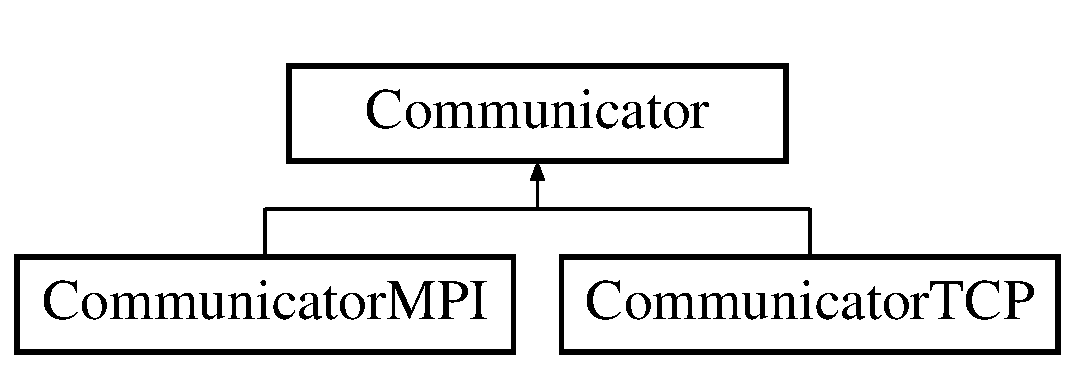
\includegraphics[height=2.000000cm]{classCommunicator}
\end{center}
\end{figure}
\subsection*{Public Member Functions}
\begin{DoxyCompactItemize}
\item 
\hypertarget{classCommunicator_a92ad155222aeafd1e5b1bd129809c2e9}{{\bfseries Communicator} (int type\-\_\-)}\label{classCommunicator_a92ad155222aeafd1e5b1bd129809c2e9}

\item 
\hypertarget{classCommunicator_a0a90cca12dcfb5721e9ac334e79c8802}{virtual int {\bfseries send} (const char $\ast$buf, int count, M\-D\-I\-\_\-\-Datatype datatype)=0}\label{classCommunicator_a0a90cca12dcfb5721e9ac334e79c8802}

\item 
\hypertarget{classCommunicator_af8618383684b7f2e1cea1a40acd43a81}{virtual int {\bfseries recv} (char $\ast$buf, int count, M\-D\-I\-\_\-\-Datatype datatype)=0}\label{classCommunicator_af8618383684b7f2e1cea1a40acd43a81}

\end{DoxyCompactItemize}


The documentation for this class was generated from the following files\-:\begin{DoxyCompactItemize}
\item 
/home/tbarnes/mdi/molssi\-\_\-driver\-\_\-interface/molssi\-\_\-driver\-\_\-interface/\hyperlink{communicator_8h}{communicator.\-h}\item 
/home/tbarnes/mdi/molssi\-\_\-driver\-\_\-interface/molssi\-\_\-driver\-\_\-interface/\hyperlink{communicator_8cpp}{communicator.\-cpp}\end{DoxyCompactItemize}

\hypertarget{classCommunicatorMPI}{\section{Communicator\-M\-P\-I Class Reference}
\label{classCommunicatorMPI}\index{Communicator\-M\-P\-I@{Communicator\-M\-P\-I}}
}
Inheritance diagram for Communicator\-M\-P\-I\-:\begin{figure}[H]
\begin{center}
\leavevmode
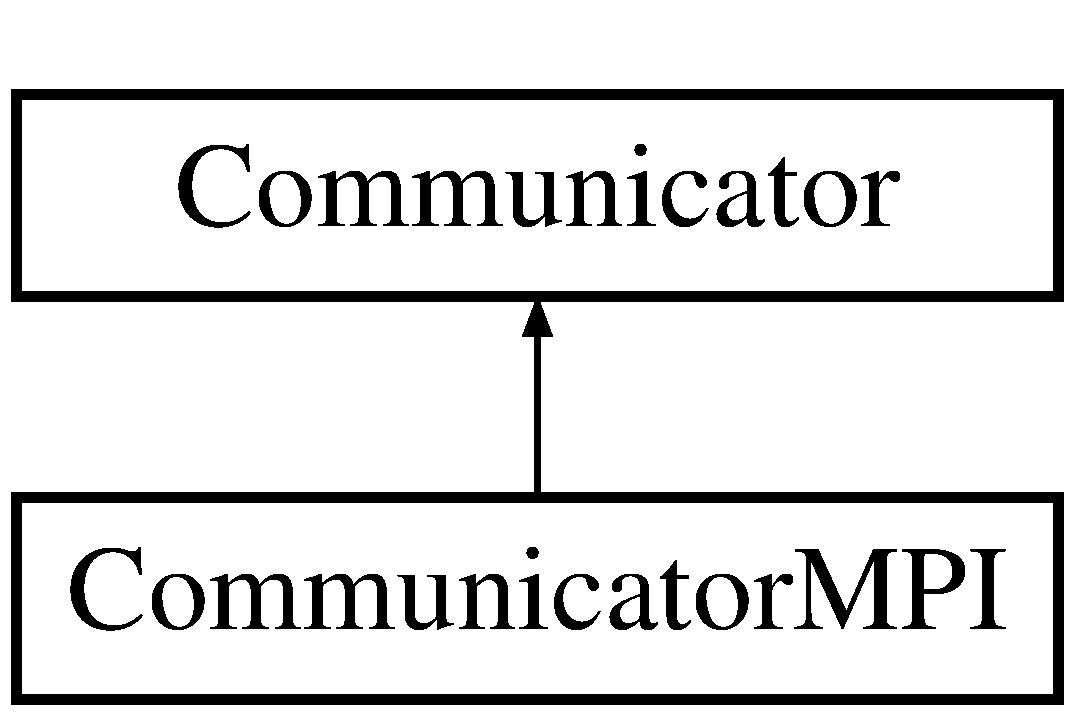
\includegraphics[height=2.000000cm]{classCommunicatorMPI}
\end{center}
\end{figure}
\subsection*{Public Member Functions}
\begin{DoxyCompactItemize}
\item 
\hypertarget{classCommunicatorMPI_aa07167a7e2dcebc0c9050ce1c18f3f32}{{\bfseries Communicator\-M\-P\-I} (int type\-\_\-, int mpi\-\_\-comm\-\_\-, int mpi\-\_\-rank\-\_\-)}\label{classCommunicatorMPI_aa07167a7e2dcebc0c9050ce1c18f3f32}

\item 
\hypertarget{classCommunicatorMPI_afd20883bec05ee4a5d97154a731a13cb}{int {\bfseries send} (const char $\ast$buf, int count, M\-D\-I\-\_\-\-Datatype datatype)}\label{classCommunicatorMPI_afd20883bec05ee4a5d97154a731a13cb}

\item 
\hypertarget{classCommunicatorMPI_ab0852541ca8f78fd3fc32e167386d76d}{int {\bfseries recv} (char $\ast$buf, int count, M\-D\-I\-\_\-\-Datatype datatype)}\label{classCommunicatorMPI_ab0852541ca8f78fd3fc32e167386d76d}

\end{DoxyCompactItemize}


The documentation for this class was generated from the following files\-:\begin{DoxyCompactItemize}
\item 
/home/tbarnes/mdi/molssi\-\_\-driver\-\_\-interface/molssi\-\_\-driver\-\_\-interface/\hyperlink{communicator_8h}{communicator.\-h}\item 
/home/tbarnes/mdi/molssi\-\_\-driver\-\_\-interface/molssi\-\_\-driver\-\_\-interface/\hyperlink{communicator_8cpp}{communicator.\-cpp}\end{DoxyCompactItemize}

\hypertarget{classCommunicatorTCP}{\section{Communicator\-T\-C\-P Class Reference}
\label{classCommunicatorTCP}\index{Communicator\-T\-C\-P@{Communicator\-T\-C\-P}}
}
Inheritance diagram for Communicator\-T\-C\-P\-:\begin{figure}[H]
\begin{center}
\leavevmode
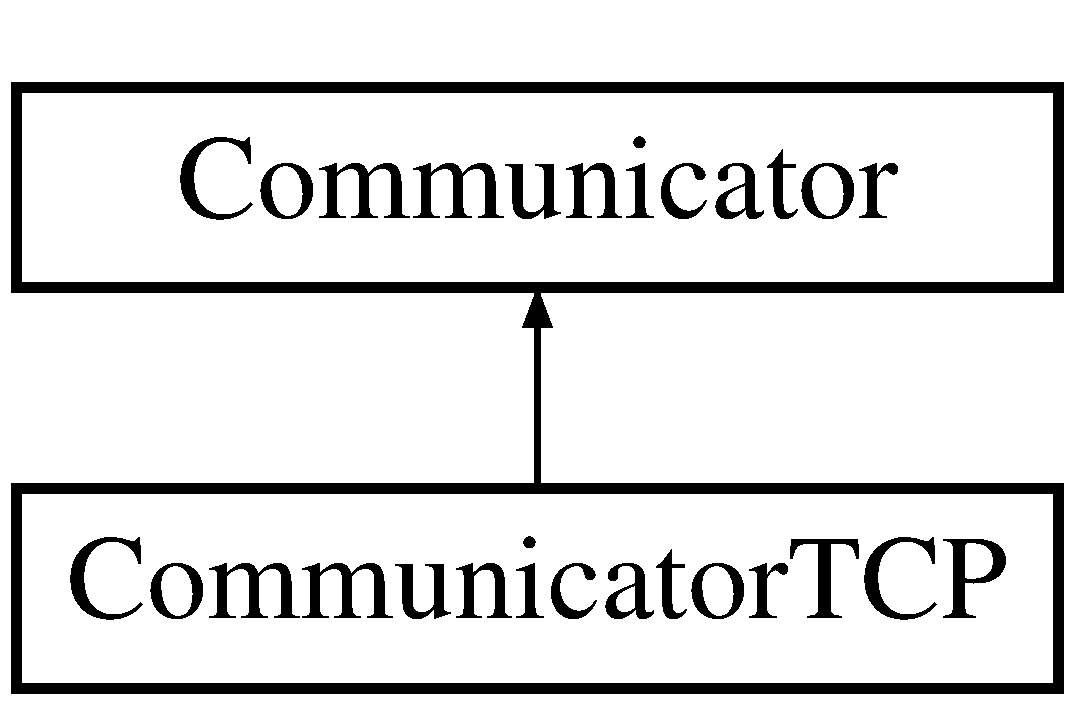
\includegraphics[height=2.000000cm]{classCommunicatorTCP}
\end{center}
\end{figure}
\subsection*{Public Member Functions}
\begin{DoxyCompactItemize}
\item 
\hypertarget{classCommunicatorTCP_a62b8536c01d0e5d3c7ab38df98a9a873}{{\bfseries Communicator\-T\-C\-P} (int type\-\_\-, int sockfd\-\_\-)}\label{classCommunicatorTCP_a62b8536c01d0e5d3c7ab38df98a9a873}

\item 
\hypertarget{classCommunicatorTCP_ac8e4894a12e34596ec7e78ab875933bf}{int {\bfseries send} (const char $\ast$buf, int count, M\-D\-I\-\_\-\-Datatype datatype)}\label{classCommunicatorTCP_ac8e4894a12e34596ec7e78ab875933bf}

\item 
\hypertarget{classCommunicatorTCP_a69d90c24e7bee5736c634565bdebab0d}{int {\bfseries recv} (char $\ast$buf, int count, M\-D\-I\-\_\-\-Datatype datatype)}\label{classCommunicatorTCP_a69d90c24e7bee5736c634565bdebab0d}

\end{DoxyCompactItemize}


The documentation for this class was generated from the following files\-:\begin{DoxyCompactItemize}
\item 
/home/tbarnes/mdi/molssi\-\_\-driver\-\_\-interface/molssi\-\_\-driver\-\_\-interface/\hyperlink{communicator_8h}{communicator.\-h}\item 
/home/tbarnes/mdi/molssi\-\_\-driver\-\_\-interface/molssi\-\_\-driver\-\_\-interface/\hyperlink{communicator_8cpp}{communicator.\-cpp}\end{DoxyCompactItemize}

\hypertarget{classmdi}{\section{mdi Module Reference}
\label{classmdi}\index{mdi@{mdi}}
}
\subsection*{Data Types}
\begin{DoxyCompactItemize}
\item 
interface \hyperlink{interfacemdi_1_1MDI__Accept__Connection__}{M\-D\-I\-\_\-\-Accept\-\_\-\-Connection\-\_\-}
\item 
interface \hyperlink{interfacemdi_1_1MDI__Listen__}{M\-D\-I\-\_\-\-Listen\-\_\-}
\item 
interface \hyperlink{interfacemdi_1_1MDI__MPI__Comm__}{M\-D\-I\-\_\-\-M\-P\-I\-\_\-\-Comm\-\_\-}
\item 
interface \hyperlink{interfacemdi_1_1mdi__recv}{mdi\-\_\-recv}
\item 
interface \hyperlink{interfacemdi_1_1MDI__Recv__}{M\-D\-I\-\_\-\-Recv\-\_\-}
\item 
interface \hyperlink{interfacemdi_1_1MDI__Recv__Command__}{M\-D\-I\-\_\-\-Recv\-\_\-\-Command\-\_\-}
\item 
interface \hyperlink{interfacemdi_1_1MDI__Request__Connection__}{M\-D\-I\-\_\-\-Request\-\_\-\-Connection\-\_\-}
\item 
interface \hyperlink{interfacemdi_1_1mdi__send}{mdi\-\_\-send}
\item 
interface \hyperlink{interfacemdi_1_1MDI__Send__}{M\-D\-I\-\_\-\-Send\-\_\-}
\item 
interface \hyperlink{interfacemdi_1_1MDI__Send__Command__}{M\-D\-I\-\_\-\-Send\-\_\-\-Command\-\_\-}
\end{DoxyCompactItemize}
\subsection*{Public Member Functions}
\begin{DoxyCompactItemize}
\item 
\hypertarget{classmdi_abb29b2ed5c592d2c5e4585ca14ae9c69}{subroutine {\bfseries mdi\-\_\-listen} (fmethod, options, fworld\-\_\-comm, ierr)}\label{classmdi_abb29b2ed5c592d2c5e4585ca14ae9c69}

\item 
\hypertarget{classmdi_ae6b39060c3cc856f240b5239a87a63d8}{subroutine {\bfseries mdi\-\_\-request\-\_\-connection} (fmethod, foptions, fworld\-\_\-comm, comm)}\label{classmdi_ae6b39060c3cc856f240b5239a87a63d8}

\item 
\hypertarget{classmdi_a5f9df9a8c58f50163196ee7ce57d63d6}{subroutine {\bfseries mdi\-\_\-accept\-\_\-connection} (connection)}\label{classmdi_a5f9df9a8c58f50163196ee7ce57d63d6}

\item 
\hypertarget{classmdi_a127a7303cd7217c0d0d646e10b188f39}{subroutine {\bfseries mdi\-\_\-mpi\-\_\-comm} (comm, ierr)}\label{classmdi_a127a7303cd7217c0d0d646e10b188f39}

\item 
\hypertarget{classmdi_a83a8409162740c37f82776526e19d4cf}{subroutine {\bfseries mdi\-\_\-send\-\_\-s} (fstring, len, type, sockfd, ierr)}\label{classmdi_a83a8409162740c37f82776526e19d4cf}

\item 
\hypertarget{classmdi_ad5a7755632e8712b6d5609e2486b184a}{subroutine {\bfseries mdi\-\_\-send\-\_\-d} (fdata, len, type, sockfd, ierr)}\label{classmdi_ad5a7755632e8712b6d5609e2486b184a}

\item 
\hypertarget{classmdi_a57bcbe45a8445f19b02126f904b43774}{subroutine {\bfseries mdi\-\_\-send\-\_\-dv} (fdata, len, type, sockfd, ierr)}\label{classmdi_a57bcbe45a8445f19b02126f904b43774}

\item 
\hypertarget{classmdi_a9451f9ead8226273424cb7efbef245c3}{subroutine {\bfseries mdi\-\_\-send\-\_\-i} (fdata, len, type, sockfd, ierr)}\label{classmdi_a9451f9ead8226273424cb7efbef245c3}

\item 
\hypertarget{classmdi_add16db0836d8e0f3cfe310e175e8243c}{subroutine {\bfseries mdi\-\_\-send\-\_\-iv} (fdata, len, type, sockfd, ierr)}\label{classmdi_add16db0836d8e0f3cfe310e175e8243c}

\item 
\hypertarget{classmdi_a78af4fc262563d2d8820a3a7cbfe0a92}{subroutine {\bfseries mdi\-\_\-recv\-\_\-s} (fstring, len, type, sockfd, ierr)}\label{classmdi_a78af4fc262563d2d8820a3a7cbfe0a92}

\item 
\hypertarget{classmdi_a557c30482625b71f46ee392d70426014}{subroutine {\bfseries mdi\-\_\-recv\-\_\-d} (fdata, len, type, sockfd, ierr)}\label{classmdi_a557c30482625b71f46ee392d70426014}

\item 
\hypertarget{classmdi_a66dc1c9e1462e5c53bd36c720aa12a38}{subroutine {\bfseries mdi\-\_\-recv\-\_\-dv} (fdata, len, type, sockfd, ierr)}\label{classmdi_a66dc1c9e1462e5c53bd36c720aa12a38}

\item 
\hypertarget{classmdi_a50204266766bbd60ec46f697309b9c5c}{subroutine {\bfseries mdi\-\_\-recv\-\_\-i} (fdata, len, type, sockfd, ierr)}\label{classmdi_a50204266766bbd60ec46f697309b9c5c}

\item 
\hypertarget{classmdi_adb59292b64be533922c3bd55c04df653}{subroutine {\bfseries mdi\-\_\-recv\-\_\-iv} (fdata, len, type, sockfd, ierr)}\label{classmdi_adb59292b64be533922c3bd55c04df653}

\item 
\hypertarget{classmdi_a9b4dc2e960271e8779e842b9e1edc0dd}{subroutine {\bfseries mdi\-\_\-send\-\_\-command} (fstring, sockfd, ierr)}\label{classmdi_a9b4dc2e960271e8779e842b9e1edc0dd}

\item 
\hypertarget{classmdi_a3a3b366cde72e01a9d3a928e902e58d0}{subroutine {\bfseries mdi\-\_\-recv\-\_\-command} (fstring, sockfd, ierr)}\label{classmdi_a3a3b366cde72e01a9d3a928e902e58d0}

\end{DoxyCompactItemize}
\subsection*{Public Attributes}
\begin{DoxyCompactItemize}
\item 
\hypertarget{classmdi_accae5b01e087f8738d86006e68417f6d}{integer, dimension(c, name=\char`\"{}mdi\-\_\-kelvin\-\_\-to\-\_\-hartree\char`\"{}), \\*
protected {\bfseries bind}}\label{classmdi_accae5b01e087f8738d86006e68417f6d}

\item 
\hypertarget{classmdi_a476a171077b89b7bc1e0153edaee118a}{integer, protected {\bfseries mdi\-\_\-command\-\_\-length}}\label{classmdi_a476a171077b89b7bc1e0153edaee118a}

\item 
\hypertarget{classmdi_a8038fa45863d082fafb692e8bc1f4b5a}{integer, protected {\bfseries mdi\-\_\-name\-\_\-length}}\label{classmdi_a8038fa45863d082fafb692e8bc1f4b5a}

\item 
\hypertarget{classmdi_ae85ef43174229bd688543ad4bcc08a2b}{integer, protected {\bfseries mdi\-\_\-int}}\label{classmdi_ae85ef43174229bd688543ad4bcc08a2b}

\item 
\hypertarget{classmdi_a69ba399f9ad46c8ac033b26574c9b6ef}{integer, protected {\bfseries mdi\-\_\-double}}\label{classmdi_a69ba399f9ad46c8ac033b26574c9b6ef}

\item 
\hypertarget{classmdi_a5741adbde5b79f06a9b94b17c7f16eb7}{integer, protected {\bfseries mdi\-\_\-char}}\label{classmdi_a5741adbde5b79f06a9b94b17c7f16eb7}

\item 
\hypertarget{classmdi_a1605c457efb88fc7e1f169734c58b52c}{integer, protected {\bfseries mdi\-\_\-tcp}}\label{classmdi_a1605c457efb88fc7e1f169734c58b52c}

\item 
\hypertarget{classmdi_a4039d7ab89098798e98dda20ece81eaf}{integer, protected {\bfseries mdi\-\_\-mpi}}\label{classmdi_a4039d7ab89098798e98dda20ece81eaf}

\item 
\hypertarget{classmdi_aff013df9c91a218d860486ff0fc757e4}{real(kind=8), dimension(c, \\*
name=\char`\"{}mdi\-\_\-kelvin\-\_\-to\-\_\-hartree\char`\"{}), \\*
protected {\bfseries bind}}\label{classmdi_aff013df9c91a218d860486ff0fc757e4}

\item 
\hypertarget{classmdi_af74f78803c251e23cd5022a8df7abc1e}{real(kind=8), protected {\bfseries mdi\-\_\-meter\-\_\-to\-\_\-bohr}}\label{classmdi_af74f78803c251e23cd5022a8df7abc1e}

\item 
\hypertarget{classmdi_a6abac217d729188855210e9327333578}{real(kind=8), protected {\bfseries mdi\-\_\-angstrom\-\_\-to\-\_\-bohr}}\label{classmdi_a6abac217d729188855210e9327333578}

\item 
\hypertarget{classmdi_a583e3421719bbf0bd951f455a0032766}{real(kind=8), protected {\bfseries mdi\-\_\-second\-\_\-to\-\_\-aut}}\label{classmdi_a583e3421719bbf0bd951f455a0032766}

\item 
\hypertarget{classmdi_ad350838a7aea84b6eca15da72d3ee4fc}{real(kind=8), protected {\bfseries mdi\-\_\-picosecond\-\_\-to\-\_\-aut}}\label{classmdi_ad350838a7aea84b6eca15da72d3ee4fc}

\item 
\hypertarget{classmdi_ace10d5db76cf54244d54b62e77b9d9a6}{real(kind=8), protected {\bfseries mdi\-\_\-newton\-\_\-to\-\_\-auf}}\label{classmdi_ace10d5db76cf54244d54b62e77b9d9a6}

\item 
\hypertarget{classmdi_a0b4e777d36fe90d506f70b16abb1b910}{real(kind=8), protected {\bfseries mdi\-\_\-joule\-\_\-to\-\_\-hartree}}\label{classmdi_a0b4e777d36fe90d506f70b16abb1b910}

\item 
\hypertarget{classmdi_a12a5c4e648f84d60dd261349d5e2cf37}{real(kind=8), protected {\bfseries mdi\-\_\-kj\-\_\-to\-\_\-hartree}}\label{classmdi_a12a5c4e648f84d60dd261349d5e2cf37}

\item 
\hypertarget{classmdi_a761336e719b236672a145cf86a8b7c95}{real(kind=8), protected {\bfseries mdi\-\_\-kjpermol\-\_\-to\-\_\-hartree}}\label{classmdi_a761336e719b236672a145cf86a8b7c95}

\item 
\hypertarget{classmdi_a2a5635f450c619dabb104846fd972b22}{real(kind=8), protected {\bfseries mdi\-\_\-kcalpermol\-\_\-to\-\_\-hartree}}\label{classmdi_a2a5635f450c619dabb104846fd972b22}

\item 
\hypertarget{classmdi_a02fe8f5658dc9d6379ceb2cc40b24b56}{real(kind=8), protected {\bfseries mdi\-\_\-ev\-\_\-to\-\_\-hartree}}\label{classmdi_a02fe8f5658dc9d6379ceb2cc40b24b56}

\item 
\hypertarget{classmdi_a4eefaa8b0fe9c708b1ba69ae86bac95c}{real(kind=8), protected {\bfseries mdi\-\_\-rydberg\-\_\-to\-\_\-hartree}}\label{classmdi_a4eefaa8b0fe9c708b1ba69ae86bac95c}

\item 
\hypertarget{classmdi_a5fc09af33b0b858f96014b3f9fdd7ee5}{real(kind=8), protected {\bfseries mdi\-\_\-kelvin\-\_\-to\-\_\-hartree}}\label{classmdi_a5fc09af33b0b858f96014b3f9fdd7ee5}

\end{DoxyCompactItemize}


The documentation for this module was generated from the following file\-:\begin{DoxyCompactItemize}
\item 
/home/tbarnes/mdi/molssi\-\_\-driver\-\_\-interface/molssi\-\_\-driver\-\_\-interface/mdi\-\_\-f90.\-f90\end{DoxyCompactItemize}

\hypertarget{interfacemdi_1_1MDI__Accept__Communicator__}{\section{mdi\-:\-:M\-D\-I\-\_\-\-Accept\-\_\-\-Communicator\-\_\- Interface Reference}
\label{interfacemdi_1_1MDI__Accept__Communicator__}\index{mdi\-::\-M\-D\-I\-\_\-\-Accept\-\_\-\-Communicator\-\_\-@{mdi\-::\-M\-D\-I\-\_\-\-Accept\-\_\-\-Communicator\-\_\-}}
}
\subsection*{Public Member Functions}
\begin{DoxyCompactItemize}
\item 
\hypertarget{interfacemdi_1_1MDI__Accept__Communicator___af692624300292e68edf192a9379e4182}{integer(kind=c\-\_\-int) function {\bfseries mdi\-\_\-accept\-\_\-communicator\-\_\-} ()}\label{interfacemdi_1_1MDI__Accept__Communicator___af692624300292e68edf192a9379e4182}

\end{DoxyCompactItemize}


The documentation for this interface was generated from the following file\-:\begin{DoxyCompactItemize}
\item 
/home/tbarnes/mdi/molssi\-\_\-driver\-\_\-interface/molssi\-\_\-driver\-\_\-interface/mdi\-\_\-f90.\-f90\end{DoxyCompactItemize}

\hypertarget{interfacemdi_1_1MDI__Conversion__Factor__}{\section{mdi\-:\-:M\-D\-I\-\_\-\-Conversion\-\_\-\-Factor\-\_\- Interface Reference}
\label{interfacemdi_1_1MDI__Conversion__Factor__}\index{mdi\-::\-M\-D\-I\-\_\-\-Conversion\-\_\-\-Factor\-\_\-@{mdi\-::\-M\-D\-I\-\_\-\-Conversion\-\_\-\-Factor\-\_\-}}
}
\subsection*{Public Member Functions}
\begin{DoxyCompactItemize}
\item 
\hypertarget{interfacemdi_1_1MDI__Conversion__Factor___acad6a9822471076622182f03b6073c77}{real(kind=c\-\_\-double) function {\bfseries mdi\-\_\-conversion\-\_\-factor\-\_\-} (in\-\_\-unit, out\-\_\-unit)}\label{interfacemdi_1_1MDI__Conversion__Factor___acad6a9822471076622182f03b6073c77}

\end{DoxyCompactItemize}


The documentation for this interface was generated from the following file\-:\begin{DoxyCompactItemize}
\item 
/home/tbarnes/mdi/molssi\-\_\-driver\-\_\-interface/molssi\-\_\-driver\-\_\-interface/mdi\-\_\-f90.\-f90\end{DoxyCompactItemize}

\hypertarget{interfacemdi_1_1MDI__Init__}{}\doxysection{mdi\+::M\+D\+I\+\_\+\+Init\+\_\+ Interface Reference}
\label{interfacemdi_1_1MDI__Init__}\index{mdi::MDI\_Init\_@{mdi::MDI\_Init\_}}
\doxysubsection*{Public Member Functions}
\begin{DoxyCompactItemize}
\item 
\mbox{\Hypertarget{interfacemdi_1_1MDI__Init___a6d3a67f8175464baa0a4e54caecfa2ae}\label{interfacemdi_1_1MDI__Init___a6d3a67f8175464baa0a4e54caecfa2ae}} 
integer(kind=c\+\_\+int) function {\bfseries mdi\+\_\+init\+\_\+} (options, world\+\_\+comm)
\end{DoxyCompactItemize}


The documentation for this interface was generated from the following file\+:\begin{DoxyCompactItemize}
\item 
/\+Users/tbarnes/\+Documents/mdi/molssi\+\_\+driver\+\_\+interface/molssi\+\_\+driver\+\_\+interface/mdi\+\_\+f90.\+f90\end{DoxyCompactItemize}

\hypertarget{interfacemdi_1_1mdi__recv}{\section{mdi\-:\-:mdi\-\_\-recv Interface Reference}
\label{interfacemdi_1_1mdi__recv}\index{mdi\-::mdi\-\_\-recv@{mdi\-::mdi\-\_\-recv}}
}
\subsection*{Public Member Functions}
\begin{DoxyCompactItemize}
\item 
\hypertarget{interfacemdi_1_1mdi__recv_a7311db44b9a07e51819c43cdb4a454bf}{subroutine {\bfseries mdi\-\_\-recv\-\_\-s} (fbuf, count, datatype, comm, ierr)}\label{interfacemdi_1_1mdi__recv_a7311db44b9a07e51819c43cdb4a454bf}

\item 
\hypertarget{interfacemdi_1_1mdi__recv_ac0a9b1a924c7106d0a574e15a5882291}{subroutine {\bfseries mdi\-\_\-recv\-\_\-d} (fbuf, count, datatype, comm, ierr)}\label{interfacemdi_1_1mdi__recv_ac0a9b1a924c7106d0a574e15a5882291}

\item 
\hypertarget{interfacemdi_1_1mdi__recv_ad5fc789a537ac5781f5d2590d7cd34d5}{subroutine {\bfseries mdi\-\_\-recv\-\_\-dv} (fbuf, count, datatype, comm, ierr)}\label{interfacemdi_1_1mdi__recv_ad5fc789a537ac5781f5d2590d7cd34d5}

\item 
\hypertarget{interfacemdi_1_1mdi__recv_a026f22dc4ed36c50764c7dc2cdfe9bd1}{subroutine {\bfseries mdi\-\_\-recv\-\_\-i} (fbuf, count, datatype, comm, ierr)}\label{interfacemdi_1_1mdi__recv_a026f22dc4ed36c50764c7dc2cdfe9bd1}

\item 
\hypertarget{interfacemdi_1_1mdi__recv_abe214d15e6c082d38999a36fb8d33fea}{subroutine {\bfseries mdi\-\_\-recv\-\_\-iv} (fbuf, count, datatype, comm, ierr)}\label{interfacemdi_1_1mdi__recv_abe214d15e6c082d38999a36fb8d33fea}

\end{DoxyCompactItemize}


The documentation for this interface was generated from the following file\-:\begin{DoxyCompactItemize}
\item 
/home/tbarnes/mdi/molssi\-\_\-driver\-\_\-interface/molssi\-\_\-driver\-\_\-interface/mdi\-\_\-f90.\-f90\end{DoxyCompactItemize}

\hypertarget{interfacemdi_1_1MDI__Recv__}{\section{mdi\-:\-:M\-D\-I\-\_\-\-Recv\-\_\- Interface Reference}
\label{interfacemdi_1_1MDI__Recv__}\index{mdi\-::\-M\-D\-I\-\_\-\-Recv\-\_\-@{mdi\-::\-M\-D\-I\-\_\-\-Recv\-\_\-}}
}
\subsection*{Public Member Functions}
\begin{DoxyCompactItemize}
\item 
\hypertarget{interfacemdi_1_1MDI__Recv___a8a02f4e2009b1219ed101b4b2c2584ed}{integer(kind=c\-\_\-int) function {\bfseries mdi\-\_\-recv\-\_\-} (buf, count, datatype, comm)}\label{interfacemdi_1_1MDI__Recv___a8a02f4e2009b1219ed101b4b2c2584ed}

\end{DoxyCompactItemize}


The documentation for this interface was generated from the following file\-:\begin{DoxyCompactItemize}
\item 
/home/tbarnes/mdi/molssi\-\_\-driver\-\_\-interface/molssi\-\_\-driver\-\_\-interface/mdi\-\_\-f90.\-f90\end{DoxyCompactItemize}

\hypertarget{interfacemdi_1_1MDI__Recv__Command__}{}\doxysection{mdi\+::M\+D\+I\+\_\+\+Recv\+\_\+\+Command\+\_\+ Interface Reference}
\label{interfacemdi_1_1MDI__Recv__Command__}\index{mdi::MDI\_Recv\_Command\_@{mdi::MDI\_Recv\_Command\_}}
\doxysubsection*{Public Member Functions}
\begin{DoxyCompactItemize}
\item 
\mbox{\Hypertarget{interfacemdi_1_1MDI__Recv__Command___a22b67734eebe9ccf72cd71a8894c28e4}\label{interfacemdi_1_1MDI__Recv__Command___a22b67734eebe9ccf72cd71a8894c28e4}} 
integer(kind=c\+\_\+int) function {\bfseries mdi\+\_\+recv\+\_\+command\+\_\+} (buf, comm)
\end{DoxyCompactItemize}


The documentation for this interface was generated from the following file\+:\begin{DoxyCompactItemize}
\item 
/\+Users/tbarnes/\+Documents/mdi/\+M\+D\+I\+\_\+\+Library/\+M\+D\+I\+\_\+\+Library/mdi\+\_\+f90.\+f90\end{DoxyCompactItemize}

\hypertarget{interfacemdi_1_1mdi__send}{}\doxysection{mdi\+::mdi\+\_\+send Interface Reference}
\label{interfacemdi_1_1mdi__send}\index{mdi::mdi\_send@{mdi::mdi\_send}}
\doxysubsection*{Public Member Functions}
\begin{DoxyCompactItemize}
\item 
\mbox{\Hypertarget{interfacemdi_1_1mdi__send_abd109b0b0e0b3f95e9782cf01d8ab7bb}\label{interfacemdi_1_1mdi__send_abd109b0b0e0b3f95e9782cf01d8ab7bb}} 
subroutine {\bfseries mdi\+\_\+send\+\_\+s} (fbuf, count, datatype, comm, ierr)
\item 
\mbox{\Hypertarget{interfacemdi_1_1mdi__send_a609eb3114aba823f801636fc4013165c}\label{interfacemdi_1_1mdi__send_a609eb3114aba823f801636fc4013165c}} 
subroutine {\bfseries mdi\+\_\+send\+\_\+d} (fbuf, count, datatype, comm, ierr)
\item 
\mbox{\Hypertarget{interfacemdi_1_1mdi__send_a891088c993f8f958c97ab01f4a504a42}\label{interfacemdi_1_1mdi__send_a891088c993f8f958c97ab01f4a504a42}} 
subroutine {\bfseries mdi\+\_\+send\+\_\+dv} (fbuf, count, datatype, comm, ierr)
\item 
\mbox{\Hypertarget{interfacemdi_1_1mdi__send_ab11c98611174127b27f723aef2055f64}\label{interfacemdi_1_1mdi__send_ab11c98611174127b27f723aef2055f64}} 
subroutine {\bfseries mdi\+\_\+send\+\_\+i} (fbuf, count, datatype, comm, ierr)
\item 
\mbox{\Hypertarget{interfacemdi_1_1mdi__send_a2890417bf9b36440044e97ddfb3a448c}\label{interfacemdi_1_1mdi__send_a2890417bf9b36440044e97ddfb3a448c}} 
subroutine {\bfseries mdi\+\_\+send\+\_\+iv} (fbuf, count, datatype, comm, ierr)
\end{DoxyCompactItemize}


The documentation for this interface was generated from the following file\+:\begin{DoxyCompactItemize}
\item 
/\+Users/tbarnes/\+Documents/mdi/\+M\+D\+I\+\_\+\+Library/\+M\+D\+I\+\_\+\+Library/mdi\+\_\+f90.\+f90\end{DoxyCompactItemize}

\hypertarget{interfacemdi_1_1MDI__Send__}{}\doxysection{mdi\+::M\+D\+I\+\_\+\+Send\+\_\+ Interface Reference}
\label{interfacemdi_1_1MDI__Send__}\index{mdi::MDI\_Send\_@{mdi::MDI\_Send\_}}
\doxysubsection*{Public Member Functions}
\begin{DoxyCompactItemize}
\item 
\mbox{\Hypertarget{interfacemdi_1_1MDI__Send___a56b7aefaad39a2e38c76f253fdf76a6b}\label{interfacemdi_1_1MDI__Send___a56b7aefaad39a2e38c76f253fdf76a6b}} 
integer(kind=c\+\_\+int) function {\bfseries mdi\+\_\+send\+\_\+} (buf, count, datatype, comm)
\end{DoxyCompactItemize}


The documentation for this interface was generated from the following file\+:\begin{DoxyCompactItemize}
\item 
/\+Users/tbarnes/\+Documents/mdi/molssi\+\_\+driver\+\_\+interface/molssi\+\_\+driver\+\_\+interface/mdi\+\_\+f90.\+f90\end{DoxyCompactItemize}

\hypertarget{interfacemdi_1_1MDI__Send__Command__}{}\doxysection{mdi\+::M\+D\+I\+\_\+\+Send\+\_\+\+Command\+\_\+ Interface Reference}
\label{interfacemdi_1_1MDI__Send__Command__}\index{mdi::MDI\_Send\_Command\_@{mdi::MDI\_Send\_Command\_}}
\doxysubsection*{Public Member Functions}
\begin{DoxyCompactItemize}
\item 
\mbox{\Hypertarget{interfacemdi_1_1MDI__Send__Command___ad79374503988a8b76342367a2b38feb5}\label{interfacemdi_1_1MDI__Send__Command___ad79374503988a8b76342367a2b38feb5}} 
integer(kind=c\+\_\+int) function {\bfseries mdi\+\_\+send\+\_\+command\+\_\+} (buf, comm)
\end{DoxyCompactItemize}


The documentation for this interface was generated from the following file\+:\begin{DoxyCompactItemize}
\item 
/\+Users/tbarnes/\+Documents/mdi/molssi\+\_\+driver\+\_\+interface/molssi\+\_\+driver\+\_\+interface/mdi\+\_\+f90.\+f90\end{DoxyCompactItemize}

\chapter{File Documentation}
\hypertarget{communicator_8cpp}{\section{/home/tbarnes/mdi/molssi\-\_\-driver\-\_\-interface/molssi\-\_\-driver\-\_\-interface/communicator.cpp File Reference}
\label{communicator_8cpp}\index{/home/tbarnes/mdi/molssi\-\_\-driver\-\_\-interface/molssi\-\_\-driver\-\_\-interface/communicator.\-cpp@{/home/tbarnes/mdi/molssi\-\_\-driver\-\_\-interface/molssi\-\_\-driver\-\_\-interface/communicator.\-cpp}}
}


Class definition for handling communication between connect codes.  


{\ttfamily \#include $<$mpi.\-h$>$}\\*
{\ttfamily \#include $<$stdio.\-h$>$}\\*
{\ttfamily \#include $<$stdlib.\-h$>$}\\*
{\ttfamily \#include $<$unistd.\-h$>$}\\*
{\ttfamily \#include \char`\"{}mdi\-\_\-global.\-h\char`\"{}}\\*
{\ttfamily \#include \char`\"{}communicator.\-h\char`\"{}}\\*
\subsection*{Variables}
\begin{DoxyCompactItemize}
\item 
\hypertarget{communicator_8cpp_a1806a2b57b24b2dd653eb4475758e5d2}{vector$<$ \hyperlink{classCommunicator}{Communicator} $\ast$ $>$ {\bfseries communicators}}\label{communicator_8cpp_a1806a2b57b24b2dd653eb4475758e5d2}

\end{DoxyCompactItemize}


\subsection{Detailed Description}
Class definition for handling communication between connect codes. 
\hypertarget{communicator_8h}{}\doxysection{/\+Users/tbarnes/\+Documents/mdi/\+M\+D\+I\+\_\+\+Library/\+M\+D\+I\+\_\+\+Library/communicator.h File Reference}
\label{communicator_8h}\index{/Users/tbarnes/Documents/mdi/MDI\_Library/MDI\_Library/communicator.h@{/Users/tbarnes/Documents/mdi/MDI\_Library/MDI\_Library/communicator.h}}


Class declaration for handling communication between connected codes.  


{\ttfamily \#include $<$mpi.\+h$>$}\newline
{\ttfamily \#include \char`\"{}mdi.\+h\char`\"{}}\newline
\doxysubsection*{Classes}
\begin{DoxyCompactItemize}
\item 
struct \mbox{\hyperlink{structcommunicator__struct}{communicator\+\_\+struct}}
\item 
struct \mbox{\hyperlink{structdynamic__array__struct}{dynamic\+\_\+array\+\_\+struct}}
\end{DoxyCompactItemize}
\doxysubsection*{Typedefs}
\begin{DoxyCompactItemize}
\item 
\mbox{\Hypertarget{communicator_8h_a7f1369263a8fc2bfc5c3f69302d4dea7}\label{communicator_8h_a7f1369263a8fc2bfc5c3f69302d4dea7}} 
typedef struct \mbox{\hyperlink{structcommunicator__struct}{communicator\+\_\+struct}} {\bfseries communicator}
\item 
\mbox{\Hypertarget{communicator_8h_ae301b80284ed481523c43e095398ba92}\label{communicator_8h_ae301b80284ed481523c43e095398ba92}} 
typedef struct \mbox{\hyperlink{structdynamic__array__struct}{dynamic\+\_\+array\+\_\+struct}} {\bfseries vector}
\end{DoxyCompactItemize}
\doxysubsection*{Functions}
\begin{DoxyCompactItemize}
\item 
\mbox{\Hypertarget{communicator_8h_a6c749e461a84e471bcab02d8115a1dfa}\label{communicator_8h_a6c749e461a84e471bcab02d8115a1dfa}} 
int {\bfseries vector\+\_\+init} (\mbox{\hyperlink{structdynamic__array__struct}{vector}} $\ast$v, size\+\_\+t stride)
\item 
\mbox{\Hypertarget{communicator_8h_a53e2a90f50c539f8239225d6f39c0213}\label{communicator_8h_a53e2a90f50c539f8239225d6f39c0213}} 
int {\bfseries vector\+\_\+push\+\_\+back} (\mbox{\hyperlink{structdynamic__array__struct}{vector}} $\ast$v, void $\ast$element)
\item 
\mbox{\Hypertarget{communicator_8h_a75ffb2ad4233613bd0c97d40b1c68611}\label{communicator_8h_a75ffb2ad4233613bd0c97d40b1c68611}} 
void $\ast$ {\bfseries vector\+\_\+get} (\mbox{\hyperlink{structdynamic__array__struct}{vector}} $\ast$v, int index)
\item 
\mbox{\Hypertarget{communicator_8h_ad3c615060f602d600023a678acee7e28}\label{communicator_8h_ad3c615060f602d600023a678acee7e28}} 
int {\bfseries communicator\+\_\+send} (const void $\ast$buf, int count, M\+D\+I\+\_\+\+Datatype datatype, M\+D\+I\+\_\+\+Comm comm)
\item 
\mbox{\Hypertarget{communicator_8h_a309565fdcf2cdb4a779edef5787e6fa9}\label{communicator_8h_a309565fdcf2cdb4a779edef5787e6fa9}} 
int {\bfseries communicator\+\_\+recv} (void $\ast$buf, int count, M\+D\+I\+\_\+\+Datatype datatype, M\+D\+I\+\_\+\+Comm comm)
\end{DoxyCompactItemize}
\doxysubsection*{Variables}
\begin{DoxyCompactItemize}
\item 
\mbox{\Hypertarget{communicator_8h_aae895626c3da244edb20b7ffcca7d05f}\label{communicator_8h_aae895626c3da244edb20b7ffcca7d05f}} 
\mbox{\hyperlink{structdynamic__array__struct}{vector}} {\bfseries communicators}
\end{DoxyCompactItemize}


\doxysubsection{Detailed Description}
Class declaration for handling communication between connected codes. 


\hypertarget{mdi_8cpp}{\section{/home/tbarnes/mdi/molssi\-\_\-driver\-\_\-interface/molssi\-\_\-driver\-\_\-interface/mdi.cpp File Reference}
\label{mdi_8cpp}\index{/home/tbarnes/mdi/molssi\-\_\-driver\-\_\-interface/molssi\-\_\-driver\-\_\-interface/mdi.\-cpp@{/home/tbarnes/mdi/molssi\-\_\-driver\-\_\-interface/molssi\-\_\-driver\-\_\-interface/mdi.\-cpp}}
}


Functions callable by users of the Mol\-S\-S\-I Driver Interface.  


{\ttfamily \#include $<$signal.\-h$>$}\\*
{\ttfamily \#include $<$netdb.\-h$>$}\\*
{\ttfamily \#include $<$netinet/in.\-h$>$}\\*
{\ttfamily \#include $<$stdio.\-h$>$}\\*
{\ttfamily \#include $<$stdlib.\-h$>$}\\*
{\ttfamily \#include $<$string.\-h$>$}\\*
{\ttfamily \#include $<$sys/socket.\-h$>$}\\*
{\ttfamily \#include $<$sys/types.\-h$>$}\\*
{\ttfamily \#include $<$sys/un.\-h$>$}\\*
{\ttfamily \#include $<$unistd.\-h$>$}\\*
{\ttfamily \#include $<$errno.\-h$>$}\\*
{\ttfamily \#include $<$iostream$>$}\\*
{\ttfamily \#include $<$vector$>$}\\*
{\ttfamily \#include \char`\"{}mdi.\-h\char`\"{}}\\*
{\ttfamily \#include \char`\"{}communicator.\-h\char`\"{}}\\*
{\ttfamily \#include \char`\"{}mdi\-\_\-manager.\-h\char`\"{}}\\*
{\ttfamily \#include \char`\"{}method.\-h\char`\"{}}\\*
\subsection*{Functions}
\begin{DoxyCompactItemize}
\item 
\hypertarget{mdi_8cpp_a10ceefc902b8eb71e2383d7ac95de2c7}{void {\bfseries mdi\-\_\-error} (const char $\ast$message)}\label{mdi_8cpp_a10ceefc902b8eb71e2383d7ac95de2c7}

\item 
int \hyperlink{mdi_8cpp_ae05ae377fa8de592f62c696c041b7d0a}{M\-D\-I\-\_\-\-Init} (const char $\ast$options, void $\ast$world\-\_\-comm)
\begin{DoxyCompactList}\small\item\em Initialize communication through the M\-D\-I library. \end{DoxyCompactList}\item 
M\-D\-I\-\_\-\-Comm \hyperlink{mdi_8cpp_a570557fdd42049c5e285faf546037531}{M\-D\-I\-\_\-\-Accept\-\_\-\-Communicator} ()
\begin{DoxyCompactList}\small\item\em Accept a new M\-D\-I communicator. \end{DoxyCompactList}\item 
int \hyperlink{mdi_8cpp_a5356b5fe5aca86c3390e13f8762a01e1}{M\-D\-I\-\_\-\-Send} (const char $\ast$buf, int count, M\-D\-I\-\_\-\-Datatype datatype, M\-D\-I\-\_\-\-Comm comm)
\begin{DoxyCompactList}\small\item\em Send data through the M\-D\-I connection. \end{DoxyCompactList}\item 
int \hyperlink{mdi_8cpp_ac94ed31fb09c8445b40265a89c72e006}{M\-D\-I\-\_\-\-Recv} (char $\ast$buf, int count, M\-D\-I\-\_\-\-Datatype datatype, M\-D\-I\-\_\-\-Comm comm)
\begin{DoxyCompactList}\small\item\em Receive data through the M\-D\-I connection. \end{DoxyCompactList}\item 
int \hyperlink{mdi_8cpp_a77e579331a36c3f0eb7f7ff9668e789d}{M\-D\-I\-\_\-\-Send\-\_\-\-Command} (const char $\ast$buf, M\-D\-I\-\_\-\-Comm comm)
\begin{DoxyCompactList}\small\item\em Send a command of length {\ttfamily M\-D\-I\-\_\-\-C\-O\-M\-M\-A\-N\-D\-\_\-\-L\-E\-N\-G\-T\-H} through the M\-D\-I connection. \end{DoxyCompactList}\item 
int \hyperlink{mdi_8cpp_ab03c0ea8beda690d6f796d3089cbfe15}{M\-D\-I\-\_\-\-Recv\-\_\-\-Command} (char $\ast$buf, M\-D\-I\-\_\-\-Comm comm)
\begin{DoxyCompactList}\small\item\em Receive a command of length {\ttfamily M\-D\-I\-\_\-\-C\-O\-M\-M\-A\-N\-D\-\_\-\-L\-E\-N\-G\-T\-H} through the M\-D\-I connection. \end{DoxyCompactList}\item 
double \hyperlink{mdi_8cpp_a886c1af1124f55d869a6f2b80a68c5a7}{M\-D\-I\-\_\-\-Conversion\-\_\-\-Factor} (char $\ast$in\-\_\-unit, char $\ast$out\-\_\-unit)
\begin{DoxyCompactList}\small\item\em Return a conversion factor between two units. \end{DoxyCompactList}\item 
\hypertarget{mdi_8cpp_a0accde4a79728e8eaab73632daba3c15}{int {\bfseries M\-D\-I\-\_\-\-Get\-\_\-\-M\-P\-I\-\_\-\-Code\-\_\-\-Rank} ()}\label{mdi_8cpp_a0accde4a79728e8eaab73632daba3c15}

\item 
\hypertarget{mdi_8cpp_a6290edc0924c7f9375e4cb9e0c7a7744}{void {\bfseries M\-D\-I\-\_\-\-Set\-\_\-\-M\-P\-I\-\_\-\-Intra\-\_\-\-Rank} (int rank)}\label{mdi_8cpp_a6290edc0924c7f9375e4cb9e0c7a7744}

\end{DoxyCompactItemize}
\subsection*{Variables}
\begin{DoxyCompactItemize}
\item 
\hypertarget{mdi_8cpp_ae5fcebdb64c7844358e07e880bcb15c2}{const int {\bfseries M\-D\-I\-\_\-\-C\-O\-M\-M\-A\-N\-D\-\_\-\-L\-E\-N\-G\-T\-H} = 12}\label{mdi_8cpp_ae5fcebdb64c7844358e07e880bcb15c2}

\item 
\hypertarget{mdi_8cpp_a8ca47e903a62de4298767ef3d446901d}{const int {\bfseries M\-D\-I\-\_\-\-N\-A\-M\-E\-\_\-\-L\-E\-N\-G\-T\-H} = 12}\label{mdi_8cpp_a8ca47e903a62de4298767ef3d446901d}

\item 
\hypertarget{mdi_8cpp_a96172c3cbab16d7b9e80288a7c94f241}{const M\-D\-I\-\_\-\-Comm {\bfseries M\-D\-I\-\_\-\-N\-U\-L\-L\-\_\-\-C\-O\-M\-M} = 0}\label{mdi_8cpp_a96172c3cbab16d7b9e80288a7c94f241}

\item 
\hypertarget{mdi_8cpp_ab88e0bb1563ba9fa73ffc49a704e43ad}{const int {\bfseries M\-D\-I\-\_\-\-I\-N\-T} = 0}\label{mdi_8cpp_ab88e0bb1563ba9fa73ffc49a704e43ad}

\item 
\hypertarget{mdi_8cpp_a3d0c16831c941e5b870461394bfe5c82}{const int {\bfseries M\-D\-I\-\_\-\-D\-O\-U\-B\-L\-E} = 1}\label{mdi_8cpp_a3d0c16831c941e5b870461394bfe5c82}

\item 
\hypertarget{mdi_8cpp_a508f568d6a6cba24d6015347d6c1469e}{const int {\bfseries M\-D\-I\-\_\-\-C\-H\-A\-R} = 2}\label{mdi_8cpp_a508f568d6a6cba24d6015347d6c1469e}

\item 
\hypertarget{mdi_8cpp_a1be671d11b9e0779a06a79abeceadd39}{const int {\bfseries M\-D\-I\-\_\-\-I\-N\-T\-\_\-\-N\-U\-M\-P\-Y} = 3}\label{mdi_8cpp_a1be671d11b9e0779a06a79abeceadd39}

\item 
\hypertarget{mdi_8cpp_aaf7153f9eda53a820f81f59ddb484ced}{const int {\bfseries M\-D\-I\-\_\-\-D\-O\-U\-B\-L\-E\-\_\-\-N\-U\-M\-P\-Y} = 4}\label{mdi_8cpp_aaf7153f9eda53a820f81f59ddb484ced}

\item 
\hypertarget{mdi_8cpp_aa69d77aeaab908058636a4420b02ae90}{const int {\bfseries M\-D\-I\-\_\-\-T\-C\-P} = 1}\label{mdi_8cpp_aa69d77aeaab908058636a4420b02ae90}

\item 
\hypertarget{mdi_8cpp_ac9eaa23189e2bf8a92c2136ee0112a87}{const int {\bfseries M\-D\-I\-\_\-\-M\-P\-I} = 2}\label{mdi_8cpp_ac9eaa23189e2bf8a92c2136ee0112a87}

\item 
\hypertarget{mdi_8cpp_a323937b5877ef054dc40e584ef767070}{const double {\bfseries M\-D\-I\-\_\-\-M\-E\-T\-E\-R\-\_\-\-T\-O\-\_\-\-B\-O\-H\-R} = 1.\-88972612546e10}\label{mdi_8cpp_a323937b5877ef054dc40e584ef767070}

\item 
\hypertarget{mdi_8cpp_ad7fb89aef0dfdc7caffe72d45b7d01d7}{const double {\bfseries M\-D\-I\-\_\-\-A\-N\-G\-S\-T\-R\-O\-M\-\_\-\-T\-O\-\_\-\-B\-O\-H\-R} = 1.\-88972612546}\label{mdi_8cpp_ad7fb89aef0dfdc7caffe72d45b7d01d7}

\item 
\hypertarget{mdi_8cpp_a9a119f46a44d6d6f594d44c8b897f9e8}{const double {\bfseries M\-D\-I\-\_\-\-S\-E\-C\-O\-N\-D\-\_\-\-T\-O\-\_\-\-A\-U\-T} = 4.\-1341374575751e16}\label{mdi_8cpp_a9a119f46a44d6d6f594d44c8b897f9e8}

\item 
\hypertarget{mdi_8cpp_a191439a37d783bcfd2c4e4989b5b2cde}{const double {\bfseries M\-D\-I\-\_\-\-P\-I\-C\-O\-S\-E\-C\-O\-N\-D\-\_\-\-T\-O\-\_\-\-A\-U\-T} = 4.\-1341374575751e4}\label{mdi_8cpp_a191439a37d783bcfd2c4e4989b5b2cde}

\item 
\hypertarget{mdi_8cpp_a3d051436cb3d2b9b9fb8528ecc70f1e6}{const double {\bfseries M\-D\-I\-\_\-\-N\-E\-W\-T\-O\-N\-\_\-\-T\-O\-\_\-\-A\-U\-F} = 1.\-213780478e7}\label{mdi_8cpp_a3d051436cb3d2b9b9fb8528ecc70f1e6}

\item 
\hypertarget{mdi_8cpp_ae40c10c77dccde242ad259fd26fd3619}{const double {\bfseries M\-D\-I\-\_\-\-J\-O\-U\-L\-E\-\_\-\-T\-O\-\_\-\-H\-A\-R\-T\-R\-E\-E} = 2.\-29371265835792e17}\label{mdi_8cpp_ae40c10c77dccde242ad259fd26fd3619}

\item 
\hypertarget{mdi_8cpp_a61e9917a12f86564edf9ef812d92fa4a}{const double {\bfseries M\-D\-I\-\_\-\-K\-J\-\_\-\-T\-O\-\_\-\-H\-A\-R\-T\-R\-E\-E} = 2.\-29371265835792e20}\label{mdi_8cpp_a61e9917a12f86564edf9ef812d92fa4a}

\item 
\hypertarget{mdi_8cpp_a27ea253093fdfdad5592091fe1f62870}{const double {\bfseries M\-D\-I\-\_\-\-K\-J\-P\-E\-R\-M\-O\-L\-\_\-\-T\-O\-\_\-\-H\-A\-R\-T\-R\-E\-E} = 3.\-80879947807451e-\/4}\label{mdi_8cpp_a27ea253093fdfdad5592091fe1f62870}

\item 
\hypertarget{mdi_8cpp_ae4f6e7e76d00e3222ec87ab235388435}{const double {\bfseries M\-D\-I\-\_\-\-K\-C\-A\-L\-P\-E\-R\-M\-O\-L\-\_\-\-T\-O\-\_\-\-H\-A\-R\-T\-R\-E\-E} = 1.\-5941730215480900e-\/3}\label{mdi_8cpp_ae4f6e7e76d00e3222ec87ab235388435}

\item 
\hypertarget{mdi_8cpp_ad50c706a104210c0c9d38ad2ee3b47dd}{const double {\bfseries M\-D\-I\-\_\-\-E\-V\-\_\-\-T\-O\-\_\-\-H\-A\-R\-T\-R\-E\-E} = 3.\-67493266806491e-\/2}\label{mdi_8cpp_ad50c706a104210c0c9d38ad2ee3b47dd}

\item 
\hypertarget{mdi_8cpp_a87b24c6eb5745296de8723de5cb7208d}{const double {\bfseries M\-D\-I\-\_\-\-R\-Y\-D\-B\-E\-R\-G\-\_\-\-T\-O\-\_\-\-H\-A\-R\-T\-R\-E\-E} = 0.\-5}\label{mdi_8cpp_a87b24c6eb5745296de8723de5cb7208d}

\item 
\hypertarget{mdi_8cpp_a40cfa9151564f12c5a0ebbee1697381e}{const double {\bfseries M\-D\-I\-\_\-\-K\-E\-L\-V\-I\-N\-\_\-\-T\-O\-\_\-\-H\-A\-R\-T\-R\-E\-E} = 3.\-16681050847798e-\/6}\label{mdi_8cpp_a40cfa9151564f12c5a0ebbee1697381e}

\end{DoxyCompactItemize}


\subsection{Detailed Description}
Functions callable by users of the Mol\-S\-S\-I Driver Interface. 

\subsection{Function Documentation}
\hypertarget{mdi_8cpp_a570557fdd42049c5e285faf546037531}{\index{mdi.\-cpp@{mdi.\-cpp}!M\-D\-I\-\_\-\-Accept\-\_\-\-Communicator@{M\-D\-I\-\_\-\-Accept\-\_\-\-Communicator}}
\index{M\-D\-I\-\_\-\-Accept\-\_\-\-Communicator@{M\-D\-I\-\_\-\-Accept\-\_\-\-Communicator}!mdi.cpp@{mdi.\-cpp}}
\subsubsection[{M\-D\-I\-\_\-\-Accept\-\_\-\-Communicator}]{\setlength{\rightskip}{0pt plus 5cm}M\-D\-I\-\_\-\-Comm M\-D\-I\-\_\-\-Accept\-\_\-\-Communicator (
\begin{DoxyParamCaption}
{}
\end{DoxyParamCaption}
)}}\label{mdi_8cpp_a570557fdd42049c5e285faf546037531}


Accept a new M\-D\-I communicator. 

The function returns an M\-D\-I\-\_\-\-Comm that describes a connection between two codes. If no new communicators are available, the function returns {\ttfamily M\-D\-I\-\_\-\-N\-U\-L\-L\-\_\-\-C\-O\-M\-M}. \hypertarget{mdi_8cpp_a886c1af1124f55d869a6f2b80a68c5a7}{\index{mdi.\-cpp@{mdi.\-cpp}!M\-D\-I\-\_\-\-Conversion\-\_\-\-Factor@{M\-D\-I\-\_\-\-Conversion\-\_\-\-Factor}}
\index{M\-D\-I\-\_\-\-Conversion\-\_\-\-Factor@{M\-D\-I\-\_\-\-Conversion\-\_\-\-Factor}!mdi.cpp@{mdi.\-cpp}}
\subsubsection[{M\-D\-I\-\_\-\-Conversion\-\_\-\-Factor}]{\setlength{\rightskip}{0pt plus 5cm}double M\-D\-I\-\_\-\-Conversion\-\_\-\-Factor (
\begin{DoxyParamCaption}
\item[{char $\ast$}]{in\-\_\-unit, }
\item[{char $\ast$}]{out\-\_\-unit}
\end{DoxyParamCaption}
)}}\label{mdi_8cpp_a886c1af1124f55d869a6f2b80a68c5a7}


Return a conversion factor between two units. 

The function returns the conversion factor from {\ttfamily in\-\_\-unit} to {\ttfamily out\-\_\-unit}.


\begin{DoxyParams}[1]{Parameters}
\mbox{\tt in}  & {\em in\-\_\-unit} & Name of the unit to convert from. \\
\hline
\mbox{\tt in}  & {\em out\-\_\-unit} & Name of the unit to convert to. \\
\hline
\end{DoxyParams}
\hypertarget{mdi_8cpp_ae05ae377fa8de592f62c696c041b7d0a}{\index{mdi.\-cpp@{mdi.\-cpp}!M\-D\-I\-\_\-\-Init@{M\-D\-I\-\_\-\-Init}}
\index{M\-D\-I\-\_\-\-Init@{M\-D\-I\-\_\-\-Init}!mdi.cpp@{mdi.\-cpp}}
\subsubsection[{M\-D\-I\-\_\-\-Init}]{\setlength{\rightskip}{0pt plus 5cm}int M\-D\-I\-\_\-\-Init (
\begin{DoxyParamCaption}
\item[{const char $\ast$}]{options, }
\item[{void $\ast$}]{world\-\_\-comm}
\end{DoxyParamCaption}
)}}\label{mdi_8cpp_ae05ae377fa8de592f62c696c041b7d0a}


Initialize communication through the M\-D\-I library. 

If using the \char`\"{}-\/method M\-P\-I\char`\"{} option, this function must be called by all ranks. The function returns {\ttfamily 0} on a success.


\begin{DoxyParams}[1]{Parameters}
\mbox{\tt in}  & {\em options} & Options describing the communication method used to connect to codes \\
\hline
\mbox{\tt in,out}  & {\em world\-\_\-comm} & On input, the M\-P\-I communicator that spans all of the codes. On output, the M\-P\-I communicator that spans the single code corresponding to the calling rank. Only used if the \char`\"{}-\/method M\-P\-I\char`\"{} option is provided. \\
\hline
\end{DoxyParams}
\hypertarget{mdi_8cpp_ac94ed31fb09c8445b40265a89c72e006}{\index{mdi.\-cpp@{mdi.\-cpp}!M\-D\-I\-\_\-\-Recv@{M\-D\-I\-\_\-\-Recv}}
\index{M\-D\-I\-\_\-\-Recv@{M\-D\-I\-\_\-\-Recv}!mdi.cpp@{mdi.\-cpp}}
\subsubsection[{M\-D\-I\-\_\-\-Recv}]{\setlength{\rightskip}{0pt plus 5cm}int M\-D\-I\-\_\-\-Recv (
\begin{DoxyParamCaption}
\item[{char $\ast$}]{buf, }
\item[{int}]{count, }
\item[{M\-D\-I\-\_\-\-Datatype}]{datatype, }
\item[{M\-D\-I\-\_\-\-Comm}]{comm}
\end{DoxyParamCaption}
)}}\label{mdi_8cpp_ac94ed31fb09c8445b40265a89c72e006}


Receive data through the M\-D\-I connection. 

If running with M\-P\-I, this function must be called only by rank {\ttfamily 0}. The function returns {\ttfamily 0} on a success.


\begin{DoxyParams}[1]{Parameters}
\mbox{\tt in}  & {\em buf} & Pointer to the buffer where the received data will be stored. \\
\hline
\mbox{\tt in}  & {\em count} & Number of values (integers, double precision floats, characters, etc.) to be received. \\
\hline
\mbox{\tt in}  & {\em datatype} & M\-D\-I handle (M\-D\-I\-\_\-\-I\-N\-T, M\-D\-I\-\_\-\-D\-O\-U\-B\-L\-E, M\-D\-I\-\_\-\-C\-H\-A\-R, etc.) corresponding to the type of data to be received. \\
\hline
\mbox{\tt in}  & {\em comm} & M\-D\-I communicator associated with the connection to the sending code. \\
\hline
\end{DoxyParams}
\hypertarget{mdi_8cpp_ab03c0ea8beda690d6f796d3089cbfe15}{\index{mdi.\-cpp@{mdi.\-cpp}!M\-D\-I\-\_\-\-Recv\-\_\-\-Command@{M\-D\-I\-\_\-\-Recv\-\_\-\-Command}}
\index{M\-D\-I\-\_\-\-Recv\-\_\-\-Command@{M\-D\-I\-\_\-\-Recv\-\_\-\-Command}!mdi.cpp@{mdi.\-cpp}}
\subsubsection[{M\-D\-I\-\_\-\-Recv\-\_\-\-Command}]{\setlength{\rightskip}{0pt plus 5cm}int M\-D\-I\-\_\-\-Recv\-\_\-\-Command (
\begin{DoxyParamCaption}
\item[{char $\ast$}]{buf, }
\item[{M\-D\-I\-\_\-\-Comm}]{comm}
\end{DoxyParamCaption}
)}}\label{mdi_8cpp_ab03c0ea8beda690d6f796d3089cbfe15}


Receive a command of length {\ttfamily M\-D\-I\-\_\-\-C\-O\-M\-M\-A\-N\-D\-\_\-\-L\-E\-N\-G\-T\-H} through the M\-D\-I connection. 

If running with M\-P\-I, this function must be called only by rank {\ttfamily 0}. The function returns {\ttfamily 0} on a success.


\begin{DoxyParams}[1]{Parameters}
\mbox{\tt in}  & {\em buf} & Pointer to the buffer where the received data will be stored. \\
\hline
\mbox{\tt in}  & {\em comm} & M\-D\-I communicator associated with the connection to the sending code. \\
\hline
\end{DoxyParams}
\hypertarget{mdi_8cpp_a5356b5fe5aca86c3390e13f8762a01e1}{\index{mdi.\-cpp@{mdi.\-cpp}!M\-D\-I\-\_\-\-Send@{M\-D\-I\-\_\-\-Send}}
\index{M\-D\-I\-\_\-\-Send@{M\-D\-I\-\_\-\-Send}!mdi.cpp@{mdi.\-cpp}}
\subsubsection[{M\-D\-I\-\_\-\-Send}]{\setlength{\rightskip}{0pt plus 5cm}int M\-D\-I\-\_\-\-Send (
\begin{DoxyParamCaption}
\item[{const char $\ast$}]{buf, }
\item[{int}]{count, }
\item[{M\-D\-I\-\_\-\-Datatype}]{datatype, }
\item[{M\-D\-I\-\_\-\-Comm}]{comm}
\end{DoxyParamCaption}
)}}\label{mdi_8cpp_a5356b5fe5aca86c3390e13f8762a01e1}


Send data through the M\-D\-I connection. 

If running with M\-P\-I, this function must be called only by rank {\ttfamily 0}. The function returns {\ttfamily 0} on a success.


\begin{DoxyParams}[1]{Parameters}
\mbox{\tt in}  & {\em buf} & Pointer to the data to be sent. \\
\hline
\mbox{\tt in}  & {\em count} & Number of values (integers, double precision floats, characters, etc.) to be sent. \\
\hline
\mbox{\tt in}  & {\em datatype} & M\-D\-I handle (M\-D\-I\-\_\-\-I\-N\-T, M\-D\-I\-\_\-\-D\-O\-U\-B\-L\-E, M\-D\-I\-\_\-\-C\-H\-A\-R, etc.) corresponding to the type of data to be sent. \\
\hline
\mbox{\tt in}  & {\em comm} & M\-D\-I communicator associated with the intended recipient code. \\
\hline
\end{DoxyParams}
\hypertarget{mdi_8cpp_a77e579331a36c3f0eb7f7ff9668e789d}{\index{mdi.\-cpp@{mdi.\-cpp}!M\-D\-I\-\_\-\-Send\-\_\-\-Command@{M\-D\-I\-\_\-\-Send\-\_\-\-Command}}
\index{M\-D\-I\-\_\-\-Send\-\_\-\-Command@{M\-D\-I\-\_\-\-Send\-\_\-\-Command}!mdi.cpp@{mdi.\-cpp}}
\subsubsection[{M\-D\-I\-\_\-\-Send\-\_\-\-Command}]{\setlength{\rightskip}{0pt plus 5cm}int M\-D\-I\-\_\-\-Send\-\_\-\-Command (
\begin{DoxyParamCaption}
\item[{const char $\ast$}]{buf, }
\item[{M\-D\-I\-\_\-\-Comm}]{comm}
\end{DoxyParamCaption}
)}}\label{mdi_8cpp_a77e579331a36c3f0eb7f7ff9668e789d}


Send a command of length {\ttfamily M\-D\-I\-\_\-\-C\-O\-M\-M\-A\-N\-D\-\_\-\-L\-E\-N\-G\-T\-H} through the M\-D\-I connection. 

If running with M\-P\-I, this function must be called only by rank {\ttfamily 0}. The function returns {\ttfamily 0} on a success.


\begin{DoxyParams}[1]{Parameters}
\mbox{\tt in}  & {\em buf} & Pointer to the data to be sent. \\
\hline
\mbox{\tt in}  & {\em comm} & M\-D\-I communicator associated with the intended recipient code. \\
\hline
\end{DoxyParams}

\hypertarget{mdi__global_8cpp}{\section{/home/tbarnes/mdi/molssi\-\_\-driver\-\_\-interface/molssi\-\_\-driver\-\_\-interface/mdi\-\_\-global.cpp File Reference}
\label{mdi__global_8cpp}\index{/home/tbarnes/mdi/molssi\-\_\-driver\-\_\-interface/molssi\-\_\-driver\-\_\-interface/mdi\-\_\-global.\-cpp@{/home/tbarnes/mdi/molssi\-\_\-driver\-\_\-interface/molssi\-\_\-driver\-\_\-interface/mdi\-\_\-global.\-cpp}}
}


Global parameters used by the Mol\-S\-S\-I Driver Interface.  


{\ttfamily \#include \char`\"{}mdi\-\_\-global.\-h\char`\"{}}\\*
\subsection*{Variables}
\begin{DoxyCompactItemize}
\item 
\hypertarget{mdi__global_8cpp_ae5fcebdb64c7844358e07e880bcb15c2}{const int {\bfseries M\-D\-I\-\_\-\-C\-O\-M\-M\-A\-N\-D\-\_\-\-L\-E\-N\-G\-T\-H} = 12}\label{mdi__global_8cpp_ae5fcebdb64c7844358e07e880bcb15c2}

\item 
\hypertarget{mdi__global_8cpp_a8ca47e903a62de4298767ef3d446901d}{const int {\bfseries M\-D\-I\-\_\-\-N\-A\-M\-E\-\_\-\-L\-E\-N\-G\-T\-H} = 12}\label{mdi__global_8cpp_a8ca47e903a62de4298767ef3d446901d}

\item 
\hypertarget{mdi__global_8cpp_a96172c3cbab16d7b9e80288a7c94f241}{const M\-D\-I\-\_\-\-Comm {\bfseries M\-D\-I\-\_\-\-N\-U\-L\-L\-\_\-\-C\-O\-M\-M} = 0}\label{mdi__global_8cpp_a96172c3cbab16d7b9e80288a7c94f241}

\item 
\hypertarget{mdi__global_8cpp_ab88e0bb1563ba9fa73ffc49a704e43ad}{const int {\bfseries M\-D\-I\-\_\-\-I\-N\-T} = 0}\label{mdi__global_8cpp_ab88e0bb1563ba9fa73ffc49a704e43ad}

\item 
\hypertarget{mdi__global_8cpp_a3d0c16831c941e5b870461394bfe5c82}{const int {\bfseries M\-D\-I\-\_\-\-D\-O\-U\-B\-L\-E} = 1}\label{mdi__global_8cpp_a3d0c16831c941e5b870461394bfe5c82}

\item 
\hypertarget{mdi__global_8cpp_a508f568d6a6cba24d6015347d6c1469e}{const int {\bfseries M\-D\-I\-\_\-\-C\-H\-A\-R} = 2}\label{mdi__global_8cpp_a508f568d6a6cba24d6015347d6c1469e}

\item 
\hypertarget{mdi__global_8cpp_a1be671d11b9e0779a06a79abeceadd39}{const int {\bfseries M\-D\-I\-\_\-\-I\-N\-T\-\_\-\-N\-U\-M\-P\-Y} = 3}\label{mdi__global_8cpp_a1be671d11b9e0779a06a79abeceadd39}

\item 
\hypertarget{mdi__global_8cpp_aaf7153f9eda53a820f81f59ddb484ced}{const int {\bfseries M\-D\-I\-\_\-\-D\-O\-U\-B\-L\-E\-\_\-\-N\-U\-M\-P\-Y} = 4}\label{mdi__global_8cpp_aaf7153f9eda53a820f81f59ddb484ced}

\item 
\hypertarget{mdi__global_8cpp_aa69d77aeaab908058636a4420b02ae90}{const int {\bfseries M\-D\-I\-\_\-\-T\-C\-P} = 1}\label{mdi__global_8cpp_aa69d77aeaab908058636a4420b02ae90}

\item 
\hypertarget{mdi__global_8cpp_ac9eaa23189e2bf8a92c2136ee0112a87}{const int {\bfseries M\-D\-I\-\_\-\-M\-P\-I} = 2}\label{mdi__global_8cpp_ac9eaa23189e2bf8a92c2136ee0112a87}

\item 
\hypertarget{mdi__global_8cpp_a323937b5877ef054dc40e584ef767070}{const double {\bfseries M\-D\-I\-\_\-\-M\-E\-T\-E\-R\-\_\-\-T\-O\-\_\-\-B\-O\-H\-R} = 1.\-88972612546e10}\label{mdi__global_8cpp_a323937b5877ef054dc40e584ef767070}

\item 
\hypertarget{mdi__global_8cpp_ad7fb89aef0dfdc7caffe72d45b7d01d7}{const double {\bfseries M\-D\-I\-\_\-\-A\-N\-G\-S\-T\-R\-O\-M\-\_\-\-T\-O\-\_\-\-B\-O\-H\-R} = 1.\-88972612546}\label{mdi__global_8cpp_ad7fb89aef0dfdc7caffe72d45b7d01d7}

\item 
\hypertarget{mdi__global_8cpp_a9a119f46a44d6d6f594d44c8b897f9e8}{const double {\bfseries M\-D\-I\-\_\-\-S\-E\-C\-O\-N\-D\-\_\-\-T\-O\-\_\-\-A\-U\-T} = 4.\-1341374575751e16}\label{mdi__global_8cpp_a9a119f46a44d6d6f594d44c8b897f9e8}

\item 
\hypertarget{mdi__global_8cpp_a191439a37d783bcfd2c4e4989b5b2cde}{const double {\bfseries M\-D\-I\-\_\-\-P\-I\-C\-O\-S\-E\-C\-O\-N\-D\-\_\-\-T\-O\-\_\-\-A\-U\-T} = 4.\-1341374575751e4}\label{mdi__global_8cpp_a191439a37d783bcfd2c4e4989b5b2cde}

\item 
\hypertarget{mdi__global_8cpp_a3d051436cb3d2b9b9fb8528ecc70f1e6}{const double {\bfseries M\-D\-I\-\_\-\-N\-E\-W\-T\-O\-N\-\_\-\-T\-O\-\_\-\-A\-U\-F} = 1.\-213780478e7}\label{mdi__global_8cpp_a3d051436cb3d2b9b9fb8528ecc70f1e6}

\item 
\hypertarget{mdi__global_8cpp_ae40c10c77dccde242ad259fd26fd3619}{const double {\bfseries M\-D\-I\-\_\-\-J\-O\-U\-L\-E\-\_\-\-T\-O\-\_\-\-H\-A\-R\-T\-R\-E\-E} = 2.\-29371265835792e17}\label{mdi__global_8cpp_ae40c10c77dccde242ad259fd26fd3619}

\item 
\hypertarget{mdi__global_8cpp_a61e9917a12f86564edf9ef812d92fa4a}{const double {\bfseries M\-D\-I\-\_\-\-K\-J\-\_\-\-T\-O\-\_\-\-H\-A\-R\-T\-R\-E\-E} = 2.\-29371265835792e20}\label{mdi__global_8cpp_a61e9917a12f86564edf9ef812d92fa4a}

\item 
\hypertarget{mdi__global_8cpp_a27ea253093fdfdad5592091fe1f62870}{const double {\bfseries M\-D\-I\-\_\-\-K\-J\-P\-E\-R\-M\-O\-L\-\_\-\-T\-O\-\_\-\-H\-A\-R\-T\-R\-E\-E} = 3.\-80879947807451e-\/4}\label{mdi__global_8cpp_a27ea253093fdfdad5592091fe1f62870}

\item 
\hypertarget{mdi__global_8cpp_ae4f6e7e76d00e3222ec87ab235388435}{const double {\bfseries M\-D\-I\-\_\-\-K\-C\-A\-L\-P\-E\-R\-M\-O\-L\-\_\-\-T\-O\-\_\-\-H\-A\-R\-T\-R\-E\-E} = 1.\-5941730215480900e-\/3}\label{mdi__global_8cpp_ae4f6e7e76d00e3222ec87ab235388435}

\item 
\hypertarget{mdi__global_8cpp_ad50c706a104210c0c9d38ad2ee3b47dd}{const double {\bfseries M\-D\-I\-\_\-\-E\-V\-\_\-\-T\-O\-\_\-\-H\-A\-R\-T\-R\-E\-E} = 3.\-67493266806491e-\/2}\label{mdi__global_8cpp_ad50c706a104210c0c9d38ad2ee3b47dd}

\item 
\hypertarget{mdi__global_8cpp_a87b24c6eb5745296de8723de5cb7208d}{const double {\bfseries M\-D\-I\-\_\-\-R\-Y\-D\-B\-E\-R\-G\-\_\-\-T\-O\-\_\-\-H\-A\-R\-T\-R\-E\-E} = 0.\-5}\label{mdi__global_8cpp_a87b24c6eb5745296de8723de5cb7208d}

\item 
\hypertarget{mdi__global_8cpp_a40cfa9151564f12c5a0ebbee1697381e}{const double {\bfseries M\-D\-I\-\_\-\-K\-E\-L\-V\-I\-N\-\_\-\-T\-O\-\_\-\-H\-A\-R\-T\-R\-E\-E} = 3.\-16681050847798e-\/6}\label{mdi__global_8cpp_a40cfa9151564f12c5a0ebbee1697381e}

\end{DoxyCompactItemize}


\subsection{Detailed Description}
Global parameters used by the Mol\-S\-S\-I Driver Interface. 
%--- End generated contents ---

% Index
\newpage
\phantomsection
\addcontentsline{toc}{part}{Index}
\printindex

\end{document}
